\ExerciseGroupsStart
\ExerciseSection

\begin{enumerate}
\def\labelenumi{\arabic{enumi})}
\item
  试证明 \(\mathbf{R}^n\) 与 \(\mathbf{R}\) 等势，利用康托尔定理（第 IV 章，§ 8，第 6 小节，定理 1）以及关系式 \(2^{\mathfrak{a}} \cdot 2^{\mathfrak{a}} = 2^{\mathfrak{a}}\) （它对一切无限基数 \(\mathfrak{a}\) 成立）。
\item
  存在区间 \(\mathbf{I} = [\mathrm{o},\mathrm{i}]\) （ \(\mathbf{R}\) 的）到正方形 \(\mathbf{I}\times \mathbf{I}\) （ \(\mathbf{R}^2\) 的）上的连续映射（“佩亚诺曲线”，参见习题 8）。（首先借助第 IV 章，§ 8 的习题 11 证明存在连续映射 \(f\) ，它把康托尔三分集 \(\mathbf{K}\) 映到 \(\mathbf{I}\times \mathbf{I}\) 上，然后把 \(f\) 延拓到 \(\mathbf{I}\) 上。）
\item
  设 A 与 B 是 \(R^{2}\) 的两个可数稠密子集。证明：存在 \(R^{2}\) 到其自身的同胚，它把 A 变换成 B。（首先证明：借助一个旋转，可以化归为投影 \(pr_{1}\) 与 \(pr_{2}\) 都是 A 与 B 到 R 中的单射映射的情形。然后，用一个适当的归纳程序，定义 A 到 B 上的一个双射，它决定 \(pr_{1}A\) 到 \(pr_{1}B\) 上的一个单调映射以及 \(pr_{2}A\) 到 \(pr_{2}B\) 上的一个单调映射。最后，利用第 IV 章，§ 2 的习题 11，证明这个映射是一个同胚，并且可以延拓为 \(R^{2}\) 到其自身的同胚。）由此推出：若 C 是 \(R^{2}\) 的一个子集，它的补集稠密，则 C 同胚于 \(Q^{2}\) 在 \(R^{2}\) 中的补集的一个子集。把这些结果推广到 \(R^{n}\) ，n \textgreater{} 2。
\item
  \(\mathbf{R}^n\) 的每个没有孤立点的可数子空间都同胚于有理直线 \(\mathbf{Q}\) （应用第 IV 章，§ 8 的习题 13）。
\item
  \(\mathbf{R}^n\) 的每个没有孤立点的全不连通紧子空间都同胚于康托尔三分集（利用第 IV 章，§ 8 的习题 11 与习题 12，以及第 II 章，§ 4，第 4 小节的命题 6）。
\item
  \(R^{n}\) 的子集 L 称为折线，如果存在点的有限序列 \((x_{i})_{0\leqslant i\leqslant p}\) （由 \(R^{n}\) 中的点组成），使得：若用 \(S_{i}\) 表示以 \(x_{i-1}\) 与 \(x_{i}\) 为端点的线段（ \(i\leqslant i\leqslant p\) ），则 L 是诸 \(S_{i}\) 的并，这些线段称为 L 的边。（一般地，定义同一条折线的 \(R^{n}\) 中点的有限序列有无穷多个。）折线也是 {[}o, i{]} 到 \(R^{n}\) 中的映射 u 的象：存在一个严格递增序列 \((t_{j})_{0\leqslant j\leqslant q}\) （在 {[}o, i{]} 中取值），\(t_{0}=0\) 且 \(t_{q}=1\) ，使得 u 是仿射线性映射
\end{enumerate}

\[
t \rightarrow \boldsymbol {a} _ {j} + t \boldsymbol {b} _ {j} \quad \text { for } \quad t _ {j - 1} \leqslant t \leqslant t _ {j} \quad \text { and } \quad i \leqslant j \leqslant q
\]

（这样的映射 \(u\) 称为“分段线性的”。）给定 \(\mathbf{R}^n\) 的一个非空子集 A，我们说 A 的两点 \(a, b\) 在 A 中可用折线连结，如果存在折线 \(L \subset A\) ，它由一个序列 \((x_i)_{0 \leqslant i \leqslant p}\) 定义，使得 \(x_0 = a\) 且 \(x_p = b\) 。若 A 的任意两点都能在 A 中用折线连结，则 A 是连通的。反之，若 A 是 \(\mathbf{R}^n\) 的连通开子集，证明 A 的任意两点都能在 A 中用折线连结（考察关系“ \(x\) 与 \(y\) 在 A 中可用折线连结”（它是 A 的点 \(x, y\) 之间的关系）；证明这是一个等价关系，而且它的类都是开集）；甚至可以始终假设这条折线是一些线段的并，其中每条线段都平行于某条坐标轴（同样的方法）。由此推出：若 A 是 \(\mathbf{R}^n\) 中的非空开集，则点 \(a \in A\) 的分支是 A 中能与 \(a\) 用 A 中折线连结的一切点组成的集。

\begin{enumerate}
\def\labelenumi{\arabic{enumi})}
\setcounter{enumi}{6}
\item
  设 A 是 \(R^{n}\) 中的非空连通开集（n \textgreater{} 1），并设 \((\mathrm{V}_{p})_{p \in \mathbb{N}}\) 是 \(R^{n}\) 中线性簇的一个可数族，其中每个线性簇的维数都 \(\leqslant n - 2\) 。证明：若 B 是诸 \(V_{p}\) 的并，则 \(A \cap \mathfrak{C}B\) 在 A 中稠密且连通。（为证明 \(A \cap \mathfrak{C}B\) 在 A 中稠密，对 n 用归纳法。然后证明：若 x, y 是 A 的两个不同的点，则对每个 \(\varepsilon > 0\) 存在点 \(y' \in A\) 满足 \(||y' - y|| \leqslant \varepsilon\) ，并且以 x 与 \(y'\) 为端点的闭线段与 B 只交于点 x。最后利用习题 6 证明 \(A \cap \mathfrak{C}B\) 连通。）
\item
  由习题 7 推出：若 \(n > \mathbf{I}\) ，则 \(\mathbf{R}^n\) 的非空开子集不与 \(\mathbf{R}\) 的任何子集同胚（*）。
\item
  \(\mathbf{R}^{n}\ (n > \mathrm{i})\) 中的折线 L（习题 6）称为简单折线，如果它同胚于 R 的区间 \(I = [0, i]\)。这等价于说存在 I 到 L 上的一个分段线性同胚 u（习题 6）。证明：若 A 是 \(\mathbf{R}^2\) 中的连通开集，且 \(\mathbf{L}\subset\mathbf{A}\) 是简单折线，则 \(\mathbf{A}-\mathbf{L}\) 连通（对组成 L 的线段的个数用归纳法论证，并利用第 I 章，§ 11 的习题 6）。
\end{enumerate}

* 10) a) 设 M 是有限集，R \(x, y\) 是 M 的元素 x, y 之间的一个对称关系。假设 M 中存在两个不同的元素 a, b，它们具有下列性质：存在 x ≠ a 与 y ≠ b，使得 x（相应地 y）是使 R \(a, z\) （相应地 R \(b, z\) ）为真的唯一的元素 z ∈ M；并且对 M 中每个异于 a 与 b 的 t，使 R \(t, z\) 为真的所有 z ∈ M 组成的集是一个由两个都异于 t 的元素组成的集。证明：在这些条件下，存在一个双射 i → x\_i （从 N 的区间 {[}o, n{]} 到 M 上），使得 x\_0 = a，x\_n = b，并且对 i ≤ i ≤ n，R \(x_{i-1}, x_i\) 为真（对 i 用归纳法定义 x\_i）。

\begin{enumerate}
\def\labelenumi{\alph{enumi})}
\setcounter{enumi}{1}
\tightlist
\item
  在 \(\mathbf{R}^n\) （ \(n \geqslant 2\) ）中——把它与 \(\mathbf{R}^{n-1} \times \mathbf{R}\) 等同起来——设 \(\mathbf{L}\) 与 \(\mathbf{L}'\) 是两条折线，分别由序列 \((\boldsymbol{x}_i)_{0 \leqslant i \leqslant p}\) 与 \((\boldsymbol{x}_j')_{0 \leqslant j \leqslant q}\) 定义，且具有下列性质：(i) 若记 \(\boldsymbol{x}_i = (\boldsymbol{y}_i, z_i)\) ，\(\boldsymbol{x}_j' = (\boldsymbol{y}_j', z_j')\) ，则我们有 \(z_0 = z_0' = 0\) ，\(z_p = z_q' = 1\) ，且 \(0 < z_i < 1\) 对 \(1 \leqslant i \leqslant p - 1\) 成立，\(0 < z_j' < 1\) 对 \(1 \leqslant j \leqslant q - 1\) 成立；(ii) \(p + q - 2\) 个数 \(z_i, z_j'\) （ \(1 \leqslant i \leqslant p - 1\) ，\(1 \leqslant j \leqslant q - 1\) ）两两不同；(iii) \(\mathbf{L}\) （相应地 \(\mathbf{L}'\) ）的两条不同的边至多有一个公共点{[}这个点可以是、也可以不是诸 \(\boldsymbol{x}_i\) （相应地 \(\boldsymbol{x}_j'\) ）之一{]}。证明：存在两个满射的分段线性映射（习题 6）\(\boldsymbol{u}\) ： \(\mathbf{I} \to \mathbf{L}\) ，\(\boldsymbol{u}'\colon \mathbf{I} \to \mathbf{L}'\) ，其中 \(\mathbf{I}\) 是区间 \([0, 1]\) （ \(\mathbf{R}\) 中的），使得：若记 \(\boldsymbol{u}(t) = (\boldsymbol{v}(t), \zeta(t))\) ，\(\boldsymbol{u}'(t) = (\boldsymbol{v}'(t), \zeta'(t))\) （ \(t \in \mathbf{I}\) ），则我们有 \(\zeta(t) = \zeta'(t)\) （对一切 \(t \in \mathbf{I}\) ），
\end{enumerate}

\[
\zeta (\mathrm{o}) = \zeta^ {\prime} (\mathrm{o}) = \mathrm{o} \quad \text { and } \quad \zeta (\mathrm{i}) = \zeta^ {\prime} (\mathrm{i}) = \mathrm{i}.
\]

{[}设 \((a_{k})_{1\leqslant k\leqslant p + q - 2}\) 是由异于 o 与 i 的诸 \(z_{i}\) 与诸 \(z_j^{\prime}\) 组成的严格递增序列，并令 \(a_0 = 0\) ，\(a_{p + q - 1} = \mathrm{i}\) ；设 \(\mathbf{B}_i\) 表示由满足下列条件的所有 \(\pmb {x} = (\pmb {y},z)\in \mathbb{R}^n\) 组成的集：

\[
a _ {i - 1} \leqslant z \leqslant a _ {i} \quad (\mathrm{I} \leqslant i \leqslant p + q - \mathrm{I});
\]

设 \(\mathfrak{M}\) 表示所有偶 \(\gamma = (\mathrm{C},\mathrm{C}^{\prime})\) 组成的集，其中 \(\mathrm{C}\) （相应地 \(\mathrm{C}'\) ）是同一个 \(\mathbf{B}_i\) 与 \(\mathbf{L}\) （相应地 \(\mathbf{L}'\) ）的一条边的交，且 \(\mathbf{C}\) 与 \(\mathbf{C}'\) 都不由单独一个点组成；又设 \(\mathbf{R}\wr \alpha, \beta\wr\) 表示元素 \(\alpha, \beta\) （ \(\mathfrak{M}\) 的）之间的下述关系：“ \(\alpha \neq \beta\) ；若 \(\alpha = (\mathrm{C}_1,\mathrm{C}_1')\) ，\(\beta = (\mathrm{C}_2,\mathrm{C}_2')\) ，则 \(\mathrm{C}_1 \cap \mathrm{C}_2\) 与 \(\mathrm{C}_1' \cap \mathrm{C}_2'\) 都非空，其中之一由单独一个点组成，而且若这个点不是诸 \(x_i\) （相应地 \(x_j'\) ）之一，则 \(\mathrm{C}_1\) 与 \(\mathrm{C}_2\) （相应地 \(\mathrm{C}_1'\) 与 \(\mathrm{C}_2'\) ）都含于 \(\mathbf{L}\) （相应地 \(\mathbf{L}'\) ）的同一条边中。证明 \(a\) ) 可应用于关系 \(\mathbf{R}.\) {]}

\begin{enumerate}
\def\labelenumi{\alph{enumi})}
\setcounter{enumi}{2}
\tightlist
\item
  在 \(\mathbf{R}^n\) 中（把它与 \(\mathbf{R}^{n-1} \times \mathbf{R}\) 等同起来），设 \(\mathbf{K}\) 是连通紧集，使得 \(\mathbf{K} \cap (\mathbf{R}^{n-1} \times \{\mathbf{o}\})\) 至少含两个不同的点。证明：若 \(\mathbf{K}' = \mathbf{K} - \mathbf{K}\) （即所有 \(x - y\) 组成的集，其中 \(x \in \mathbf{K}\) 且 \(y \in \mathbf{K}\) ），则 \(\mathbf{K}' \cap (\mathbf{R}^{n-1} \times \{\mathbf{o}\})\) 含有一个不由单独一个点组成的连通集。{[}利用 b)，并应用第 II 章，§ 4 的命题 6 与习题 15。{]}
\end{enumerate}

\begin{enumerate}
\def\labelenumi{\arabic{enumi})}
\setcounter{enumi}{10}
\tightlist
\item
  把第 IV 章，§ 8 的习题 14 与习题 15 推广到空间 \(\mathbf{R}^n\) （ \(n \geqslant 2\) ）。
\end{enumerate}

* 12) a) 设 \(f\) 是 \(\mathbf{R}\) 到 \(\mathbf{R}\) 中的映射，并设 \(\mathbf{G} \subset \mathbf{R}^2\) 是 \(f\) 的图象。假设 \(\mathbf{G}\) 在 \(\mathbf{R}^2\) 中稠密，并且与 \(\mathbf{R}^2\) 中每个不完全含于形如 \(\{x_n\} \times \mathbf{R}\) 的直线的可数并中的完全集相交。证明 \(\mathbf{G}\) 连通。（若不然，证明：存在两个非空的不相交开集 \(\mathbf{A}\) ，\(\mathbf{B}\) （ \(\mathbf{R}^2\) 中的），使得 \(\mathbf{G}\) 是 \(\mathbf{G} \cap \mathbf{A}\) 与 \(\mathbf{G} \cap \mathbf{B}\) 的并，\(\mathbf{A}\) 中至少有一点与 \(\mathbf{B}\) 中的一点有相同的横坐标（利用 \(\mathbf{R}\) 连通这一事实）；然后利用习题 11。）

\begin{enumerate}
\def\labelenumi{\alph{enumi})}
\setcounter{enumi}{1}
\tightlist
\item
  由 a) 推出：存在 R 到 R 中的线性映射 f，它的图象 G 在 \(R^{2}\) 中稠密且连通。{[}利用 a) 与习题 11，按照《集合论》第 III 章，§ 6 习题 24 中的同样方法，用超限归纳法定义 f 在 R 的一个哈梅尔基的各点上的值。{]}由此推出：\(R^{2}\) 的子群 G 满足第 V 章，§ 3 习题 4 中的条件 ( \(R_{I}\) ) 与 ( \(R_{II}\) ) ，但不是局部紧的，因而它的拓扑严格细于 R 的通常拓扑；并且 G 不是局部连通的。
\end{enumerate}

\begin{enumerate}
\def\labelenumi{\arabic{enumi})}
\setcounter{enumi}{12}
\tightlist
\item
  把 \(R^{n}\) 与 \(R^{n-1} \times R\) 等同起来，设 f 是 \(R^{n-1}\) 的一个开子集 A 到 R 中的连续映射，并设 S 是它的图象。证明：\(R^{n}\) 的子空间 S 同胚于 A，并且 S 在“圆柱” \(A \times R\) 中的补集是 \(A \times R\) 中的稠密开集，而且当 A 连通时它恰有两个分支。
\end{enumerate}

\ExerciseSection

* 1) 设 \(\mathbf{I}\) 是 \(\mathbf{R}^n\) 中的闭立方体，它是 \(n\) 个都等于 \([-\frac{1}{2}\pi, \frac{1}{2}\pi]\) 的区间之积。对每个点 \(x = (x_i)\) （属于 \(\mathbf{I}\) ），我们使它对应于满足下列条件的点 \(y = (y_j)\) （ \(\mathbf{R}^{n+1}\) 中的）：

\[
y _ {1} = \sin x _ {1}
\]

\[
{y _ {2}} {= \cos x _ {1} \sin x _ {2}}
\]

\[
y _ {p} = \cos x _ {1} \cos x _ {2} \dots \cos x _ {p - 1} \sin x _ {p} (2 \leqslant p \leqslant n - 1)
\]

\[
y _ {n} = \cos x _ {1} \cos x _ {2} \dots \cos x _ {n - 1} \sin 2 x _ {n}
\]

\[
y _ {n + 1} = \cos x _ {1} \cos x _ {2} \dots \cos x _ {n - 1} \cos 2 x _ {n}.
\]

证明：I 在这个映射下的象是球面 \(S_{n}\) ，并且这个映射在 I 的内部上的限制是到 \(S_{n}\) 中一个稠密开集上的同胚。 *

\begin{enumerate}
\def\labelenumi{\arabic{enumi})}
\setcounter{enumi}{1}
\tightlist
\item
  定义 \(\mathbf{S}_p \times \mathbf{S}_q\) 到 \(\mathbf{S}_{p + q + 1}\) 的一个子集上的同胚{[}注意 \(\mathbf{S}_{p + q + 1}\) 的方程是
\end{enumerate}

\[
\left. \left(x _ {1} ^ {2} + \dots + x _ {p + 1} ^ {2}\right) + \left(x _ {p + 2} ^ {2} + \dots + x _ {p + q + 2} ^ {2}\right) = \mathrm{I} \right].
\]

\begin{enumerate}
\def\labelenumi{\arabic{enumi})}
\setcounter{enumi}{2}
\tightlist
\item
  \begin{enumerate}
  \def\labelenumii{\alph{enumii})}
  \tightlist
  \item
    证明：若 \(f\) 是 \(\mathbf{S}_1\) 到 \(\mathbf{R}^n\) 中的连续映射，则 \(f\) 可以延拓为 \(\mathbf{B}_2\) 到 \(\mathbf{R}^n\) 中的连续映射{[}把点 \(tx \in \mathbf{B}_2\) （ \(t \geqslant 0\) ，\(x \in S_1\) ）映为 \(tf(x)\) {]}。
  \end{enumerate}
\end{enumerate}

\begin{enumerate}
\def\labelenumi{\alph{enumi})}
\setcounter{enumi}{1}
\tightlist
\item
  由此推出：若 \(f\) 是 \(\mathbf{S}_1\) 到 \(\mathbf{S}_n\) 中的连续映射，满足 \(f(\mathbf{S}_1) \neq \mathbf{S}_n\) ，则 \(f\) 可以延拓为 \(\mathbf{B}_2\) 到 \(\mathbf{S}_n\) 中的连续映射{[}利用一个其顶点不属于 \(f(\mathbf{S}_1)\) 的球极投影{]}。(*)
\end{enumerate}

\begin{enumerate}
\def\labelenumi{\arabic{enumi})}
\setcounter{enumi}{3}
\tightlist
\item
  证明：不存在 \(S_{1}\) 到 R 中的同胚。（注意 \(S_{1}\) 中任一点在 \(S_{1}\) 中的补集是连通的，而 R 的每个连通子集是一个区间。）
\end{enumerate}

由此推出：\(S_{1}\) 到 \(S_{1}\) 的一个子空间上的同胚必然是 \(S_{1}\) 到 \(S_{1}\) 上的同胚（利用第 4 小节的命题 4）。

\begin{enumerate}
\def\labelenumi{\arabic{enumi})}
\setcounter{enumi}{4}
\item
  证明：若 \(n > 1\) ，则球面 \(\mathbf{S}_n\) 不同胚于圆周 \(\mathbf{S}_1\) （参见 § 1 的习题 8）。
\item
  把 \(S_{1}\) 与环面 T（即 R 关于关系 \(x \equiv y \pmod{1}\) 的商，第 4 小节命题 4 的推论 2）等同起来，设 \(\varphi\) 表示 R 到 \(S_{1}\) 上的典范映射。拓扑空间 E 到 \(S_{1}\) 中的连续映射 f 称为非本质的，如果存在 E 到 R 中的连续映射 g，使得 \(f = \varphi \circ g\) 。(**) 不是非本质的映射称为本质映射。
\end{enumerate}

证明 \(S_{1}\) 到 \(S_{1}\) 上的恒等映射是本质映射（利用习题 4）。

\begin{enumerate}
\def\labelenumi{\arabic{enumi})}
\setcounter{enumi}{6}
\item
  证明：存在 \(S_{1}\) 的一致结构的一个围域 U，使得只要 f 是拓扑空间 E 到 \(S_{1}\) 中的非本质映射，则每个连续映射 \(f' : E \to S_{1}\) （它使 \((f(x), f'(x)) \in U\) 对一切 \(x \in E\) 成立）也是非本质的。
\item
  证明：不存在连续映射 \(f\) ：它把 \(\mathbf{B}_2\) 映到 \(\mathbf{S}_1\) 上并延拓 \(\mathbf{S}_1\) 的恒等映射（利用习题 7，证明 \(f\) 限制在以 o 为中心、以 \(r \leqslant i\) 为半径的圆周上时，总是该圆周到 \(S_{1}\) 中的非本质映射，从而当 \(r = i\) 时得出矛盾）。
\item
  设 E 是含多于一个点的拓扑空间。证明：存在 \(S_{1}\) 到 \(F = E \times S_{1}\) 中的连续映射 f，满足 \(f(S_{1}) \neq F\) ，并且它不能延拓为 \(B_{2}\) 到 F 中的连续映射（利用习题 8）。由此推出：若 n \textgreater{} 1 ，则 \(S_{n}\) 、\(R^{n}\) 与 \(B_{n}\) 都不同胚于任何形如 \(E \times S_{1}\) 的空间，其中 E 是任意拓扑空间（参见习题 3）。特别地，若 n \textgreater{} 1 ，\(S_{n}\) 不同胚于 \(S_{1}^{n}\) ，而且对一切 n，\(B_{n}\) 不同胚于 \(S_{1}^{n}\) 。
\end{enumerate}

同样证明：\(R^{2}\) 不同胚于 \(R^{2}\) 中一点的补集，且 \(S_{2}\) 不同胚于 \(B_{2}\) （若不真，\(R^{2}\) 将同胚于 \(S_{1}\) 与区间 \([0, 1]\) 的乘积）。

\begin{enumerate}
\def\labelenumi{\arabic{enumi})}
\setcounter{enumi}{9}
\tightlist
\item
  设 \(H_{n,p,q}\) 表示 \(R^{n}\) 中由方程
\end{enumerate}

\[
x _ {1} ^ {2} + x _ {2} ^ {2} + \dots + x _ {p} ^ {2} - x _ {p + 1} ^ {2} - \dots - x _ {p + q} ^ {2} = \mathrm{I} \quad (p + q \leqslant n).
\]

所定义的“二次超曲面”。证明 \(\mathbf{H}_{n,p,q}\) 同胚于 \(\mathbf{S}_{p - 1}\times \mathbf{R}^{n - p}\) 。

\begin{enumerate}
\def\labelenumi{\arabic{enumi})}
\setcounter{enumi}{10}
\tightlist
\item
  设 \(C_{n,p}\) 是 \(R^{n}\) 中由方程
\end{enumerate}

\[
x _ {1} ^ {2} + x _ {2} ^ {2} + \dots + x _ {p} ^ {2} - x _ {p + 1} ^ {2} - \dots - x _ {n} ^ {2} = 0 \quad (\mathrm{I} \leqslant p \leqslant n - \mathrm{I}).
\]

所定义的“二次锥面”，证明 \(\{0\}\) 在 \(\mathbf{C}_{n,p}\) 中的补集同胚于 \(\mathbf{S}_{p-1} \times \mathbf{S}_{n-p-1} \times \mathbf{R}\) 。

* 12) \(\mathbf{R}^n\) 中含原点 o 的子集 E 称为（关于 o 的）星形集，如果对一切 \(x \in \mathbf{E}\) 与一切 \(t \in [0, 1]\) ，都有 \(tx \in \mathbf{E}\) 。E 与以 o 为端点的闭射线的交或者是整条射线，或者是一条以 o 为其一个端点的线段。E 的壳是指由这些线段的非零端点组成的集 K，再加上 o——如果存在一条射线，它与 E 的交仅由 o 组成。在下文中我们总假设 \(o \notin K\) 。

\begin{enumerate}
\def\labelenumi{\alph{enumi})}
\item
  证明 E 的壳含于 E 的边界。给出一个这两个集不相同的例子。
\item
  证明：若 E 的壳 K 是紧的，则存在 \(R^{n}\) 到其自身的同胚，它把 K 变换成 \(S_{n-1}\) ，把 \(\overline{E}\) 变换成 \(B_{n}\) ，并且把 E 的内部变换成 \(B_{n}\) 的内部（把每一点 \(x \in K\) 映为它在 \(S_{n-1}\) 上的中心投影，然后把这个映射延拓到整个 \(R^{n}\) 上）。由此推出：E 的边界与其壳重合，并且 E 的内部是由点 tx 组成的集，其中 \(x \in K\) 且 \(t \in [0, I[\) 。
\item
  若 E 无界且其边界与其壳重合，则 E 的内部同胚于 \(R^{n}\) ，并且它的壳 K 同胚于 \(S_{n-1}\) 的一个开子集{[}证明 E 在同胚 \(x \to x/(1 + ||x||)\) 下的象满足 b) 的条件{]}。
\item
  给出一个无界星形集 E 的例子，它的壳是闭的，但不与 E 的边界重合。
\end{enumerate}

\begin{enumerate}
\def\labelenumi{\arabic{enumi})}
\setcounter{enumi}{12}
\tightlist
\item
  证明：在空间 \(S_{n}\) 中，外部非空的非空开集的边界具有连续统的势（利用第 4 小节的命题 4）。
\end{enumerate}

\ExerciseSection

\begin{enumerate}
\def\labelenumi{\arabic{enumi})}
\tightlist
\item
  设 \(f\) 是 \(\mathbf{S}_2\) 到 \(\mathbb{R}^4\) 中的映射，满足
\end{enumerate}

\[
f \left(x _ {1}, x _ {2}, x _ {3}\right) = \left(x _ {1} ^ {2} - x _ {2} ^ {2}, x _ {1} x _ {2}, x _ {1} x _ {3}, x _ {2} x _ {3}\right).
\]

这个函数在 \(S_{2}\) 的对径点处取相同的值。证明：过渡到商后，它定义 \(P_{2}\) 到 \(R^{4}\) 的一个子空间上的一个同胚。

同样证明：由下式定义的映射 \(g\) （ \(\mathbf{S}_3\) 到 \(\mathbf{R}^6\) 中的）

\[
g \left(x _ {1}, x _ {2}, x _ {3}, x _ {4}\right) = \left(x _ {1} ^ {2} - x _ {2} ^ {2}, x _ {1} x _ {2}, x _ {1} x _ {3} + x _ {2} x _ {4}, x _ {3} ^ {2} - x _ {4} ^ {2}, x _ {3} x _ {4}, x _ {1} x _ {4} - x _ {2} x _ {3}\right)
\]

在过渡到商后定义 \(P_{3}\) 到 \(R^{6}\) 中的一个同胚。

\begin{enumerate}
\def\labelenumi{\arabic{enumi})}
\setcounter{enumi}{1}
\item
  把射影空间 \(P_{n}\) 与第 1 小节命题 3 中所定义的 \(B_{n}\) 的商空间等同起来，并设 \(\varphi\) 表示 \(B_{n}\) 到 \(P_{n}\) 上的典范映射。拓扑空间 E 到 \(P_{n}\) 中的连续映射 f 称为非本质的，如果存在 E 到 \(B_{n}\) 中的连续映射 g，使得 \(f = \varphi \circ g\) ，反之的情形则称为本质的（参见 § 2 的习题 6）。证明：存在 \(P_{n}\) 的一致结构的一个围域 U，使得若 f 是拓扑空间 E 到 \(P_{n}\) 中的一个非本质映射，则每个连续映射 \(f'\) （ E 到 \(P_{n}\) 中的，且使 \((f(x), f'(x)) \in \mathbf{U}\) 对一切 \(x \in E\) 成立）也是非本质的。
\item
  若 \(\mathbf{S}_1\) 到 \(\mathbf{P}_n\) 中的一个连续映射是本质的（习题 2），则它不能延拓为 \(\mathbf{B}_2\) 到 \(\mathbf{P}_n\) 中的连续映射（参见 § 2 的习题 8）。
\item
  若 \(n > \mathbf{1}\) ，则存在本质映射 \(f\) （ \(\mathbf{S}_1\) 到 \(\mathbf{P}_n\) 中的），使得 \(f(\mathbf{S}_1) \neq \mathbf{P}_n\) {[}取 \(f(\mathbf{S}_1)\) 为在 \(\varphi\) 之下 \(\mathbf{B}_n\) 的一条直径的象；这个象是一条射影直线{]}。由此推出，若 \(n > \mathbf{1}\) ，则 \(\mathbf{P}_n\) 既不同胚于 \(\mathbf{S}_n\) ，也不同胚于 \(\mathbf{B}_n\) （利用 § 3 的习题 3 与 § 2 的习题 3）。
\item
  若把 \(\mathbf{R}^2\) 看作嵌在 \(\tilde{\mathbf{R}} \times \tilde{\mathbf{R}}\) 中，而把 \(\mathbf{R}\) 看作嵌在 \(\tilde{\mathbf{R}}\) 中，证明映射 \((x, y) \to x + y\) （ \(\mathbf{R}^2\) 到 \(\mathbf{R}\) 中的）可以连续延拓到点 \((\infty, a)\) 与 \((a, \infty)\) （它们属于 \(\tilde{\mathbf{R}} \times \tilde{\mathbf{R}}\) ， \(a\) 取一切有限值），但不能连续延拓到 \((\infty, \infty)\) 。若把 \(\mathbf{R}^2\) 看作嵌在 \(\mathbf{P}_2\) 中（ \(\mathbf{R}\) 仍看作嵌在 \(\tilde{\mathbf{R}}\) 中），则 \(x + y\) 可以连续延拓到无穷远直线上除齐次坐标为 \((1, -1, 0)\) 的点以外的所有点。
\end{enumerate}

对乘积 xy 陈述并证明这些结果的类似命题。

\begin{enumerate}
\def\labelenumi{\arabic{enumi})}
\setcounter{enumi}{5}
\item
  若 \(n \geqslant 0\) ，设 \(\mathfrak{F}\) 是 \(\mathbf{P}_n\) 的所有闭子集所成的集合，并按第 II 章 § 2 习题 6 b) 的程序赋予由 \(\mathbf{P}_n\) 的一致结构诱导的一致结构。证明：集合 \(\mathbf{P}_{n,p}\) （由 \(p \geqslant 0\) 维射影线性簇组成）在 \(\mathfrak{F}\) 中是闭的，且在 \(\mathbf{P}_{n,p}\) 上由 \(\mathfrak{F}\) 的拓扑诱导的拓扑与第 5 小节定义 2 中所定义的拓扑相同。{[}要定义 \(\mathbf{P}_n\) 的一致结构的围域，可把 \(\mathbf{P}_n\) 看作 \(\mathbf{S}_n\) 的商空间（第 1 小节命题 2），并取 \(\mathbf{S}_n\) 的被半径趋于 o 的球所作的有限覆盖。{]}
\item
  \begin{enumerate}
  \def\labelenumii{\alph{enumii})}
  \tightlist
  \item
    证明：在第 5 小节的记号下，空间 \(\mathbf{L}_{n,p}\) 同胚于 \(\mathbf{V}_{n,p}\) 与 \(\mathbb{R}^{p(p+1)/2}\) 的乘积。注意每个矩阵 \(X\in\mathbf{L}_{n,p}\) 都可以唯一地表示成 \(U\) . \(\Upsilon\) 的形式，其中 \(\Upsilon\in\mathbf{V}_{n,p}\) ，而 \(U=(u_{ij})\) 满足 \(u_{ij}=0\) （对 \(i<j\) ），且 \(u_{ii}>0\) （对 \(\mathbf{i}\leqslant i\leqslant p\) ）。令 \(\Upsilon=f(X)\) 。
  \end{enumerate}
\end{enumerate}

\begin{enumerate}
\def\labelenumi{\alph{enumi})}
\setcounter{enumi}{1}
\tightlist
\item
  在第 5 小节命题 8 的记号下，证明 \(f\) 是 \(\mathbf{B}_{\sigma}\) 到 \(f(\mathbf{B}_{\sigma})\) 上的一个同胚{[}注意 \(X \to f(X_{\sigma}^{-1}X)\) 是 \(\mathbf{A}_{\sigma}\) 到 \(f(\mathbf{B}_{\sigma})\) 上的连续映射，且 \(f(X_{\sigma}^{-1}X)\) 与 \(X \mod \Delta_{n,p}\) 属于同一类；然后应用引理 2{]}。由此推出， \(\mathbf{D}_{\sigma}\) （即 \(\mathbf{A}_{\sigma}\) 与 \(\mathbf{V}_{n,p}\) 的交）同胚于 \(\mathbf{V}_{p,p}\) 与 \(\mathbb{R}^{p(n - p)}\) 的乘积{[}属于 \(\mathbf{D}_{\sigma}\) 的每个矩阵都可以唯一地表示成 \(\mathbf{V}_{p,p}\) 中一个矩阵与 \(f(\mathbf{B}_{\sigma})\) 中一个矩阵的乘积{]}。
\end{enumerate}

\begin{enumerate}
\def\labelenumi{\arabic{enumi})}
\setcounter{enumi}{7}
\tightlist
\item
  设 \(g\) 是这样的映射：对每个矩阵 \(X \in \mathbf{L}_{n,p}\) ， \(X'g(X)\) 是由前 \(q\) 行（取自 \(X\) ）构成的矩阵（ \(q < p\) ）。证明： \(g\) 在 \(\mathbf{V}_{n,p}\) 上的限制是 \(\mathbf{V}_{n,p}\) 到 \(\mathbf{V}_{n,q}\) 上的连续开映射{[}利用习题 7 a)，注意若 \(X = U.Y\) 则
\end{enumerate}

\[
g (X) = U ^ {\prime}. g (\Upsilon),
\]

其中 \(U'\) 是由 U 去掉指标 \textgreater q 的行与列所得的矩阵；另一方面，注意 f 是开映射{]}。

\begin{enumerate}
\def\labelenumi{\arabic{enumi})}
\setcounter{enumi}{8}
\item
  证明： \(\mathbf{V}_{n,p}\) 在 \(p < n\) 时是连通的（利用习题 8 与第 I 章 § 11 第 3 小节命题 7）。
\item
  在射影空间 \(P_{n}\) 中，设 \(H_{n,p}\) 是由方程
\end{enumerate}

\[
x _ {0} ^ {2} + x _ {1} ^ {2} + \dots + x _ {p - 1} ^ {2} - x _ {p} ^ {2} - \dots - x _ {n} ^ {2} = 0 \quad (\mathrm{I} \leqslant p \leqslant n).
\]

所定义的“二次超曲面”。证明： \(H_{n,1}\) 与 \(H_{n,n}\) 都同胚于 \(S_{n-1}\) 。若 \(2 \leqslant p \leqslant n - 1\) ，则 \(H_{n,p}\) 同胚于把乘积 \(S_{p-1} \times S_{n-p}\) （视为 \(R^{p} \times R^{n-p+1}\) 的子空间）的每个点与其对径点等同起来所得到的空间。 \(H_{n,p}\) 的每个点都有一个同胚于 \(R^{n-1}\) 的开邻域。

证明： \(H_{3,2}\) 同胚于 \(S_{1} \times S_{1}\) {[}把 \(S_{1} \times S_{1}\) 与 \(T \times T\) 等同起来， \(S_{1} \times S_{1}\) 的一对对径点与点 \((u, v)\) 和 \((1/2 + u, 1/2 + v)\) （属于 \(T \times T\) ）相等同；然后考虑映射 \((u, v) \to (u + v, u - v)\) （ \(T \times T\) 到其自身的映射）{]}。

\begin{enumerate}
\def\labelenumi{\arabic{enumi})}
\setcounter{enumi}{10}
\tightlist
\item
  在射影空间 \(P_{n}\) 中，设 \(C_{n,p}\) 是由方程
\end{enumerate}

\[
x _ {1} ^ {2} + x _ {2} ^ {2} + \dots + x _ {p} ^ {2} - x _ {p + 1} ^ {2} - \dots - x _ {n} ^ {2} = 0 \quad (\mathrm{I} \leqslant p \leqslant n - \mathrm{I}).
\]

证明： \(\{0\}\) 在 \(C_{n,p}\) 中的补集同胚于 \(\mathbf{R} \times H_{n-1,p}\) （沿用习题 10 的记号）。

\section*{历史注记}
\phantomsection
\addcontentsline{toc}{section}{历史注记}

（括号中的数字指本注记末尾的参考文献。）

我们已经有机会指出，平面和空间的解析几何的发展使数学家们得到 n 维空间的概念，这个概念为他们提供了一种极为方便的几何语言，可以简单而简洁地表达关于任意多个变量的方程的代数定理，特别是线性代数的所有一般结果。但是，尽管到 19 世纪中叶这种语言已为许多几何学家所惯用，它仍然纯粹是出于方便，而且由于缺乏三维以上空间的“直观”表示，在这类空间中似乎就排除了“依连续性”的论证——这类论证仅仅以“直观”为基础，在平面和（三维）空间中却是被允许的。黎曼在其关于位置分析（analysis situs）以及几何学基础的研究中，第一个通过与三维空间的类比使用了这类考虑（见第 I 章的历史注记）（*）；遵循他的榜样，许多数学家被鼓励去使用这类论证，并取得很大的成功，特别是在多个复变量的代数函数论中。但是，鉴于那个时期对空间直观的掌握非常有限，人们有理由对这类考虑的证明价值持怀疑态度，只允许在纯启发式的意义上使用它们，即认为它们只是使某些定理的真实性显得可信。因此，庞加莱在他 1887 年关于两个复变量的二重积分的残数的论文中，尽可能地避免求助于四维空间的直观：“Comme cette langue hypergéométrique répugne encore à beaucoup de bons esprits, je n'en ferai qu'un usage peu fréquent”；他为此目的所使用的技巧，使他在讨论三维空间时以拓扑论证为足，而对于这些论证，他不再迟疑求助于直观（{[}1{]}）。

此外，康托尔的发现，特别是断言 R 与 \(R^{n}\) 等势的那个著名定理{[}它似乎动摇了整个维数概念（*）{]}，表明为了把几何学和拓扑学建立在牢固的基础上，必须使它们完全摆脱对直观的一切依赖。我们已经指出（参见第 I 章的历史注记），这一需要是现代一般拓扑学观念的起源；但甚至在这一理论创立之前，就已经开始了对实 n 维空间及其直接推广（“n 维流形”）的拓扑学的严格研究，其所用的方法本属于拓扑学中称为“组合拓扑学”、或更好地称为“代数拓扑学”的那一分支。本丛书中将有一卷专门讨论拓扑学的这一分支，读者可以在那里找到关于其发展历史阶段的资料；在本章中我们只限于建立实数空间和实射影空间的最基本的拓扑性质，它们在历史上曾充当代数拓扑学方法的出发点。

\subsection*{参考文献}

{[}1{]} L. SCHLÄFLI, Gesammelte mathematische Abhandlungen, vol.~1, Basel (Birkhauser), 1950, pp.~169-387.

{[}2{]} H. POINCARÉ, Œuvres, vol.~3, p.~443 et seq. Paris (Gauthier-Villars) (1934) {[}Acta Mathematica, 9 (1887), p.~321{]}.

{[}3{]} G. CANTOR 与 R. DEDEKIND, Briefwechsel, Act. Sci. et Ind., no. 518, Paris (Hermann) (1937).

\chapter{\texorpdfstring{\(\mathbf{R}^n\) 的加法群}{R 的 n 次幂的加法群}}

\section{\texorpdfstring{\(\mathbf{R}^n\) 的子群与商群}{R 的 n 次幂的子群与商群}}

让我们首先引进如下的约定：若 G 是一个拓扑群，我们对 n 个都等于 G 的因子的乘积群 \(G^{n}\) （对每个整数 n \textgreater{} 0 ）已经定义过（第 III 章 § 2）。在本节中，我们要把这一定义推广到 n = 0 的情形，约定 \(G^{0}\) 表示只由一个元素组成的群。若 H 是任意群，我们将把 \(G^{0} \times H\) 与 H 等同起来。

\pandocbounded{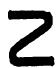
\includegraphics[keepaspectratio]{images/part001_b5dea1c7.jpg}}

在集合 \(\mathbf{R}^n\) 上，我们一方面要考虑它的（加法）拓扑群结构，另一方面要考虑它在域 \(\mathbf{R}\) 上的向量空间结构（第 VI 章 § 1 第 3 小节）。给定子集 \(\mathbf{A}\) （含于 \(\mathbf{R}^n\) ）后，我们可以考虑 \(\mathbf{R}^n\) 的由 \(\mathbf{A}\) 生成的子群（ \(\mathbf{A}\) 的点以整数为系数的一切线性组合所成的集合），同时也可以考虑由 \(\mathbf{A}\) 生成的向量子空间（ \(\mathbf{A}\) 的点以实数为系数的一切线性组合所成的集合）；必须仔细区分这两个概念。按照代数学中作出的定义， \(\mathbf{A}\) 的秩是向量子空间 \(\mathbf{V}\) （ \(\mathbf{R}^n\) 中由 \(\mathbf{A}\) 生成的）的维数；因此说 \(\mathbf{A}\) 的秩为 \(p\) ，就等价于说存在 \(p\) 个点 \(x_i \in \mathbf{A}\) ，它们关于域 \(\mathbf{R}\) 构成一个自由系（换句话说，关系 \(\sum_{i} t_i x_i = 0\) （其中 \(t_i\) 是实数）蕴涵 \(t_i = 0\) （对每个 \(i\) ）），并且构成 \(\mathbf{V}\) 的一个基（意即 \(\mathbf{V}\) 的每个点都是 \(x_i\) 以实数为系数的一个线性组合）。

在以下的内容中，我们还必须用到 \(\mathbf{R}^n\) 的点关于有理数域 \(\mathbf{Q}\) 自由这一概念；这样的系是一个有限子集 \((\pmb{x}_i)\) （ \(\mathbf{R}^n\) 的），满足关系 \(\sum_{i} r_i x_i = 0\) （其中 \(r_i\) 是有理数（或整数——这是一回事））蕴涵对每个 i 有 \(r_{i}=0\) 。这个概念必须与关于 R 的自由系的概念仔细地区分开：每个关于 R 自由的系都关于 Q 自由，但反过来不成立（例如，R 中的数 1 与 \(\sqrt{2}\) 构成关于 Q 的自由系，但不构成关于 R 的自由系）。每当我们不加限定地说到自由系时，总是指关于 R 的自由系。因此有必要在 \(R^{n}\) 上把关于 R 的向量空间结构与关于 Q 的向量空间结构区分开；特别地，由 \(R^{n}\) 的子集 A 生成的关于 Q 的向量子空间是 A 以有理数为系数的一切线性组合所成的集合 U；它含于由 A 生成的（关于 R 的）向量子空间 V，但一般与 V 不同。U（关于 Q）的维数称为 A 的有理秩；它至少等于上面定义的 A 的秩（即 V 关于 R 的维数）；若 A 是无限集，它可以是无限的，而 \(R^{n}\) 的任何非空子集的秩总 \(\leqslant n\) ；特别地， \(R^{n}\) 的任何不可数子集的有理秩总是无限的，因为 Q 上任何有限维向量空间都是可数的。

\pandocbounded{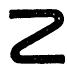
\includegraphics[keepaspectratio]{images/part001_3371d17f.jpg}}

在本节中，我们将首先确定加法群 \(R^{n}\) 的闭子群的结构。

\subsection{\texorpdfstring{\(\mathbf{R}^n\) 的离散子群}{R 的 n 次幂的离散子群}}

我们在第 V 章（§ 1 第 1 小节命题 1）中已经看到，R 的闭子群中除 R 自身外只有离散子群，它们都由单个元素生成。我们将从考虑 \(\mathbf{R}^n\) 的离散子群开始。

首先，由 \(\mathbf{R}^n\) 的典范基（第 VI 章 § 1 第 3 小节）的 \(p\) 个向量（ \(p \leqslant n\) ）所生成的 \(\mathbf{R}^n\) 的子群是一个离散群，同构于乘积 \(\mathbf{Z}^p\) ——即 \(p\) 个都等于 \(\mathbf{Z}\) 的群的乘积。更一般地，考虑子群 \(\mathbf{G}\) ，它由构成自由系的 \(p\) 个点 \(a_i\) （ \(i \leqslant i \leqslant p\) ）生成。存在 \(\mathbf{R}^n\) 到其自身上的一个双射线性映射，它把 \(a_i\) 映为 \(e_i\) （ \(i \leqslant i \leqslant p\) ）；由于这样的映射是拓扑群 \(\mathbf{R}^n\) 的自同构， \(\mathbf{G}\) 作为拓扑群同构于由 \(e_i\) （ \(i \leqslant i \leqslant p\) ）生成的子群，因此是一个秩为 \(p\) 、同构于 \(\mathbf{Z}^p\) 的离散子群。

群 \(Z^{p}\) 的结构、从而 G 的结构，已在代数学中研究过。我们回顾这一研究的主要结果。G 关于环 Z 的基是由 p 个点组成的系

\[
\boldsymbol {b} _ {i} = \sum_ {j = 1} ^ {p} r _ {i j} \boldsymbol {a} _ {j},
\]

其中 \(r_{ij}\) 是使得行列式 \(\det(r_{ij})\) 等于 +1 或 -1 的整数。G 的每个子群 H 都是离散的且秩 \(q \leqslant p;\) 此外，若 \(H\) 是给定的秩为 \(q\) 的子群，则存在由 \(p\) 个点 \(b_i\) （ \(i \leqslant i \leqslant p\) ）组成并生成 \(G\) 的自由系，以及由 \(q\) 个点 \(c_i\) （ \(i \leqslant i \leqslant q\) ）组成并生成 \(H\) 的系，使得有 \(c_i = e_i b_i\) （对 \(i \leqslant i \leqslant q\) ），其中 \(e_i\) 是整数（ \(H\) 关于 \(G\) 的不变因子），满足

\[
e _ {i + 1} \equiv o (\mathrm{mod} e _ {i}) \quad \text { for } \quad i \leqslant i \leqslant q - i.
\]

商群 G/H 是一个离散群，同构于 \(Z^{p-q} \times F\) ，其中 F 是一个有限交换群，是 q 个循环子群的直积，这些循环子群的阶分别为 \(e_{1}, \ldots, e_{q}\) 。

现在我们将证明，刚才所考虑的 \(\mathbf{R}^n\) 的离散子群是仅有的离散子群。

命题 1. 设 G 是 \(\mathbf{R}^n\) 的一个秩为 \(p\) 的离散子群， \((\boldsymbol{a}_i)_{1 \leqslant i \leqslant p}\) 是 G 的 \(p\) 个点组成的自由系，P 是以 o 为中心、以 \(\boldsymbol{a}_i\) 为基向量的闭超平行体（第 VI 章 § 1 第 3 小节）。则集合 G ∩ P 是有限的且生成 G，且 G 的每个点都是 \(\boldsymbol{a}_i\) 以有理数为系数的线性组合。

G ∩ P 是紧的且离散的，因而是有限的。设 x 是 G 的任意点；它等于线性组合 \(\sum_{i=1}^{p} t_{i}a_{i}\) （诸 \(a_{i}\) 以实数为系数）。对每个整数 m \textgreater{} 0 ，考虑点

\[
z _ {m} = m x - \sum_ {i = 1} ^ {p} [ m t _ {i} ] a _ {i} = \sum_ {i = 1} ^ {p} (m t _ {i} - [ m t _ {i} ]) a _ {i} (*);
\]

它属于 G，且由于 \(o \leqslant mt_{i} - [mt_{i}] < 1\) ，它位于 P 中。因此，首先有 \(x = z_{1} + \sum_{i=1}^{p} [t_{i}] a_{i}\) ，故 G 由 \(G \cap P\) 生成；其次，由于 \(G \cap P\) 是有限的，存在两个不同的整数 h、k，使得 \(z_{h} = z_{k}\) ，从而 \((h - k)t_{i} = [ht_{i}] - [kt_{i}]\) （对 \((1 \leqslant i \leqslant p)\) ），因此 \(t_{i}\) 是有理数。

推论. 设 \((\pmb{a}_i)_{1\leqslant i\leqslant p}\) 是 \(p\) 个点（ \(\mathbf{R}^n\) 的）组成的自由系，并设

\[
\boldsymbol {b} = \sum_ {i = 1} ^ {p} t _ {i} \boldsymbol {a} _ {i}
\]

是 \(a_{i}\) 以实数为系数的一个线性组合。则 \(R^{n}\) 中由 \(p + i\) 个点 \(a_{1}, a_{2}, \ldots, a_{p}\) 与 b 所生成的子群 G 是离散的，当且仅当诸数 \(t_{i}\) 是有理数。

命题 1 表明这条件是必要的。它也是充分的，因为若这条件满足，我们就可以写 \(t_i = m_i / d\) ，其中 \(d\) 与诸 \(m_i\) 是整数（ \(i \leqslant i \leqslant p\) ）；于是 \(b\) 是 \(p\) 个点 ( \(\mathrm{I} / d\) ) \(a_i\) 以整数为系数的线性组合；因此 \(G\) 是由这 \(p\) 个点生成的离散群的一个子群，从而本身是离散的。

命题 1 的结果可以表述如下：若 q 个点 \(x_{i}\) （ \(i \leqslant i \leqslant q\) ，属于 \(R^{n}\) 的一个离散子群 G）构成一个关于 R 相关的系，则它们构成一个关于 Q 相关的系。由此立即推出， \(R^{n}\) 的离散子群的有理秩等于它的秩。

把命题 1 的推论应用到 \(a_{i}\) 为 \(n\) 个向量 \(\pmb{e}_{i}\) （ \(\mathbf{R}^{n}\) 的典范基的）的情形，就得到下面的命题：

命题 2（克罗内克）. 设 \(\theta_{1}, \theta_{2}, \ldots, \theta_{n}\) 是 \(n\) 个实数。为了对每个 \(\varepsilon > 0\) ，存在一个整数 \(q\) 与 \(n\) 个整数

\[
p _ {i} \quad (\mathrm{I} \leqslant i \leqslant n)
\]

使得

\[
\left| q \theta_ {i} - p _ {i} \right| \leqslant \varepsilon \quad (\mathrm{I} \leqslant i \leqslant n),
\]

其中这些不等式中至少有一个的左端不为零，其充分必要条件是诸 \(\theta_{i}\) 中至少有一个是无理数。

定理 1. \(\mathbf{R}^n\) 的每个秩等于 \(p\) 的离散子群 G 都由 \(p\) 个点组成的自由系生成。

根据前面回顾过的同构于 \(Z^{p}\) 的群的性质，只需证明 G 是由 p 个点组成的自由系生成的离散群的一个子群。现在，由于 G 的秩为 p，存在 G 的由 p 个点 \(a_{i}\) （ \(1 \leqslant i \leqslant p\) ）组成的自由系，使得每个 \(x \in G\)

都等于线性组合 \(\sum_{i=1}^{p} t_i a_i\) （诸 \(a_i\) 以实数为系数）；

由于 G 是离散的，命题 1 表明诸 \(t_i\) 是有理数。此外，命题 1 表明 G 由有限多个点生成；由于这些点是 \(\boldsymbol{a}_i\) 以有理数为系数的线性组合，故存在整数 \(d\) ，使得它们是 \(p\) 个点 \((\mathrm{I}/d)\boldsymbol{a}_i = \boldsymbol{a}_i'\) 以整数为系数的线性组合。由此推出，G 是由诸 \(\boldsymbol{a}_i'\) 生成的群的一个子群。

定理 1 也可以不用不变因子理论来证明（参见习题 1）。

\(R^{n}\) 中秩为 n 的离散子群也称为 \(R^{n}\) 中的格。

\subsection{\texorpdfstring{\(\mathbf{R}^n\) 的闭子群}{R 的 n 次幂的闭子群}}

我们已经知道 \(\mathbf{R}^n\) 的闭子群的两种类型：一方面是 \(\mathbf{R}^n\) 的向量子空间，它们同构于群 \(\mathbf{R}^p\) （ \(p \leqslant n\) ）（第 IV 章 § 1 第 4 小节命题 2）；另一方面是离散子群（第 III 章 § 2 第 1 小节命题 5），如我们刚才所见，它们同构于群 \(\mathbf{Z}^q\) （ \(q \leqslant n\) ）。现在我们要确定 \(\mathbf{R}^n\) 的任意闭子群的结构，办法是证明这样一个子群同构于形如

\[
\mathbf {R} ^ {p} \times \mathbf {Z} ^ {q} \quad \text { where } \quad \mathrm{o} \leqslant p + q \leqslant n.
\]

证明基于下面的命题：

命题 3. \(\mathbf{R}^n\) 的每个非离散的闭子群都包含一条过 o 的直线。

设 \((\pmb{x}_p)_{p\in \mathbb{N}}\) 是 \(\mathbf{G}\) 的点的一个无穷序列，满足 \(\pmb{x}_p\neq 0\) 且 \(\lim_{p\to \infty}\pmb{x}_p = 0\) ；由假设这样的序列存在。设 \(\mathbf{P}\) 是以 \(0\) 为中心且包含诸 \(\pmb{x}_p\) 的开立方体。设 \(k_{p}\) 表示最大的整数 \(h > 0\) ，它使 \(h\pmb{x}_p\in \mathrm{P}\) （由于 \(\mathbf{P}\) 是有界长方体且 \(\pmb{x}_p\neq 0\) ， \(k_{p}\) 的存在性由阿基米德公理得出）。点 \(k_{p}\pmb{x}_{p}\) 位于紧集 \(\overline{\mathrm{P}}\) 中，因此序列 \((k_{p}\pmb{x}_{p})_{p\in \mathbb{N}}\) 有一个聚点 \(\pmb {a}\in \overline{\mathrm{P}}\) 。若 \(||k_p\pmb {x}_p - \pmb {a}||\leqslant \varepsilon\) ，我们有

\[
\left| \left| \left(k _ {p} + \mathrm{I}\right) x _ {p} - a \right| \right| \leqslant \varepsilon + \left| \left| x _ {p} \right| \right|,
\]

且由于 \(\lim_{p\to \infty}\boldsymbol{x}_p = 0\) ，由此得出 \(\boldsymbol{a}\) 也是序列 \(((k_p + 1)x_p)\) 的一个聚点，而这个序列的点属于闭集 \(\mathfrak{C}P\) （按 \(k_{p}\) 的定义）；因此 \(\boldsymbol{a} \in \overline{\mathrm{P}} \cap \mathfrak{C}P\) （即 P 的边界，见图 5），这蕴涵 \(\boldsymbol{a} \neq 0\) 。此外，由于 G 是闭的，我们有 \(\boldsymbol{a} \in \mathrm{G}\) 。设 \(t\) 是任意实数；由于 \(|tk_p - [tk_p]| < 1\) ，关系 \(||k_p x_p - a|| \leqslant \varepsilon\) 蕴涵 \(||[tk_p]x_p - ta|| \leqslant |t| \varepsilon + ||x_p||\) ；由于 \(\lim_{p \to \infty} x_p = 0\) ， \(ta\) 是

\pandocbounded{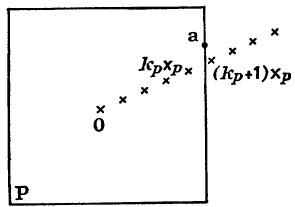
\includegraphics[keepaspectratio]{images/part001_2a0a1c84.jpg}}\\
图 5.

\pandocbounded{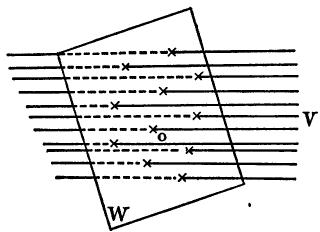
\includegraphics[keepaspectratio]{images/part001_3dc381fa.jpg}}\\
图 6.

序列 \(([tk_p]x_p)\) 的一个聚点；但这个序列的点都属于 G，因而 \(ta \in G\) ，因为 G 是闭的。证毕。

定理 2. 设 G 是 \(\mathbf{R}^n\) 的一个闭子群，其秩为 \(r\) （ \(0 \leqslant r \leqslant n\) ）。则存在含于 G 中的最大向量子空间 V；对每个与 V 互补的向量子空间 W，W ∩ G 是离散的，且 G 是 V 与 W ∩ G 的直和。

我们首先来确立 V 的存在性，办法是证明 G 中所有过 o 的直线的并集是一个向量子空间：事实上，由这些直线的并集生成的向量子空间与由它们生成的子群相同。群 G 是 V 与 W ∩ G 的直和；因为若 \(x \in G\) ，我们有 \(x = y + z\) ，其中 \(y \in V\) 且 \(z \in W\) ；由于 \(V \subset G\) ，有 \(z = x - y \in G\) ，因此 \(z \in W \cap G\) 。剩下要证明 \(W \cap G\) 是离散的；这由命题 3 得出，因为 \(W \cap G\) 是一个不含任何直线的闭子群，这是由 V 的定义推出的。

若 \(G \neq V\) ，我们可以说 G 是可数无穷多个线性簇的并，这些线性簇平行于 V 且经过离散群 \(W \cap G\) 的点（图 6）。

若 \(p\) 是向量子空间 \(\mathbf{V}\) 的维数，则 \(p \leqslant r\) ，且 \(\mathbf{W} \cap \mathbf{G}\) 是秩为 \(r - p\) 的离散群。

推论 1. 存在一个基 \((\pmb{a}_i)_{1\leqslant i\leqslant n}\) （ \(\mathbf{R}^n\) 的），使得

\[
\boldsymbol {a} _ {i} \in \mathrm{G} \quad (\mathrm{I} \leqslant i \leqslant r), \quad \boldsymbol {a} _ {i} \in \mathrm{V} \quad (\mathrm{I} \leqslant i \leqslant p)
\]

并且使得 \(\mathbf{G}\) 是形如 \(\sum_{i=1}^{p} t_i a_i + \sum_{j=p+1}^{r} n_j a_j\) 的点所成的集合，其中 \(t_i\) 取遍一切实数值，而 \(n_j\) 取遍一切整数值。

这由定理 2 以及应用于离散群 \(W \cap G\) 的第 1 小节的定理 1 得出。

推论 2. 存在 \(\mathbf{R}^n\) 的一个自同构，它把 \(\mathbf{G}\) 映到群 \(\mathbf{G}'\) 上，该群同构于 \(\mathbf{R}^p \times \mathbf{Z}^{r-p}\) ，是由 \(e_1, e_2, \ldots, e_p\) 生成的向量子空间与由 \(e_{p+1}, e_{p+2}, \ldots, e_r\) 生成的（离散）加法子群的直和。

这是推论 1 的直接推论。定理 2 的推论 2 表明， \(R^{n}\) 的闭子群 G 由两个 \(\geqslant 0\) 的整数完全确定（在相差一个同构的意义下）：它的秩，我们记作 \(r(\mathbf{G})\) ，以及含于 G 中的最大向量子空间的维数，我们称之为 G 的维数并记作 \(d(\mathbf{G})\) 。

这些整数需要满足的唯一条件是不等式 \(o \leqslant d(\mathbf{G}) \leqslant r(\mathbf{G}) \leqslant n\) 。

\subsection{相伴子群}

设 \(\mathbf{G}\) 是 \(\mathbf{R}^n\) 的任意子群（闭或不闭）。考虑集合 \(\mathbf{G}^*\) （由满足如下条件的点 \(\boldsymbol{u} = (u_i) \in \mathbf{R}^n\) 组成）：对一切 \(\boldsymbol{x} = (x_i) \in \mathbf{G}\) ，数 \((\boldsymbol{u}| \boldsymbol{x}) = \sum_{i=1}^{n} u_i x_i\) 是整数。立即可以看出， \(\mathbf{G}^*\) 是 \(\mathbf{R}^n\) 的一个子群；它称为与 \(\mathbf{G}(*)\) 相伴的子群。若 \(\mathbf{G}\) 与 \(\mathbf{H}\) 是 \(\mathbf{R}^n\) 的两个子群，且 \(\mathbf{H} \subset \mathbf{G}\) ，则显然有 \(\mathbf{G}^* \subset \mathbf{H}^*\) 。

命题 4. 子群 \(\mathbf{G}^*\) ——它与一个子群 \(\mathbf{G}\) （ \(\mathbf{R}^n\) 的）相伴——是闭的，且我们有 \((\overline{\mathbf{G}})^* = \mathbf{G}^*\) 。

对每个 \(x \in G\) ，用 \(f_x(u)\) 表示 \((u|x)\) ； \(f_x\) 是线性形式，因此是连续的。由于 \(G^*\) 是诸集合 \(f_x^{-1}(Z)\) （当 \(x\) 取遍 \(G\) 时）的交，且这些集合中的每一个都是闭的，由此得出 \(G^*\) 是闭的。另一方面，若 \(u \in G^*\) ，则有 \((u|x) \in Z\) （对一切 \(x \in G\) ），因而，由于 \(Z\) 在 \(R\) 中是闭的，有 \((u|y) \in Z\) （对一切 \(y \in \overline{G}\) ）；于是 \(u \in (G)^*\) 。但我们有 \((\overline{G})^* \subset G^*\) （因为 \(G \subset \overline{G}\) ），所以 \((\overline{G})^* = G^*\) 。

考虑 \(\mathbf{G}^*\) 在 \(\mathbf{G}\) 为闭时的结构。由第 2 小节定理 2 的推论 1，存在一个基 \((\pmb{a}_i)_{\mathbf{1} \leqslant i \leqslant n}\) （ \(\mathbf{R}^n\) 的），使得 \(\mathbf{G}\) 恰为由点

\[
\boldsymbol {x} = \sum_ {i = 1} ^ {p} t _ {i} \boldsymbol {a} _ {i} + \sum_ {j = p + 1} ^ {p + q} n _ {j} \boldsymbol {a} _ {j},
\]

所组成的集合，其中 \(t_i\) 取遍一切实数值，而 \(n_j\) 取遍一切整数值。于是 \((\boldsymbol{u}|\boldsymbol{x})\) 对所有这些点 \(\boldsymbol{x}\) 都是整数，当且仅当 \((\boldsymbol{u}|\boldsymbol{a}_i) = 0\) （对 \(1 \leqslant i \leqslant p\) ）且 \((\boldsymbol{u}|\boldsymbol{a}_i)\) 是整数（对 \(p + 1 \leqslant i \leqslant p + q\) ）。用 \((\boldsymbol{a}_i')_{1 \leqslant i \leqslant n}\) 表示 \(\mathbf{R}^n\) 的满足 \((\boldsymbol{a}_i'|\boldsymbol{a}_j) = 0\) （对 \(i \neq j\) ）的基

\[
\left(\boldsymbol {a} _ {i} ^ {\prime} \mid \boldsymbol {a} _ {i}\right) = \mathrm{I} \quad \text { for } \quad \mathrm{I} \leqslant i \leqslant n
\]

{[}即与 \((a_{i})\) “对偶”的基{]}；若置 \(u = \sum_{i=1}^{n} u_{i} a_{i}^{\prime}\) ，则显然点 \(u \in G^{*}\) 由下列条件刻画： \(u_{i} = 0\) （对 \(i \leqslant i \leqslant p\) ），且 \(u_{i} \in Z\) （对

\[
p + \mathrm{i} \leqslant i \leqslant p + q;
\]

因而 \(G^{*}\) 是一个向量子空间 W 与一个离散子群的直和，前者的基由那些 \(a_{i}^{\prime}\) （满足 \(p + q + i \leqslant i \leqslant n\) ）组成，后者由那些 \(a_{i}^{\prime}\) （满足 \(p + i \leqslant i \leqslant p + q\) ）生成。换言之：

命题 5. 对 \(\mathbf{R}^n\) 的每个闭子群 G ，

\[
r (\mathbf {G} ^ {*}) = n - d (\mathbf {G}) \quad a n d \quad d (\mathbf {G} ^ {*}) = n - r (\mathbf {G}).
\]

让我们把同样的推理应用于 \(\mathbf{G}^*\) 。注意到与 \((\pmb{a}_i')\) 对偶的基是 \((\pmb{a}_i)\) ，我们就看出：

命题 6. 对每个子群 \(\mathbf{G}\) （ \(\mathbf{R}^n\) 的），我们有 \((\mathbf{G}^*)^* = \overline{\mathbf{G}}\) 。

推论. 一点 x 位于 \(R^{n}\) 的子群 G 的闭包中，当且仅当 \((u|x)\) 对每个 \(u \in R^{n}\) 都是整数，其中 \((u|y)\) 对一切 \(y \in G\) 均为整数。

让我们把这个关于位于子群 \(\mathbf{G}\) 的闭包中的点的刻画，应用于子群 \(\mathbf{G}\) 的情形——它由 \(n\) 个向量 \(\boldsymbol{e}_j\) （ \(\mathrm{i} \leqslant j \leqslant n\) ，属于典范基）以及任意 \(m\) 个点 \(\boldsymbol{a}_i\) （ \(\mathrm{i} \leqslant i \leqslant m\) ，属于 \(\mathbf{R}^n\) ）生成。说 \((\boldsymbol{u}|\boldsymbol{e}_j)\) 对 \(\mathrm{i} \leqslant j \leqslant n\) 是整数，就意味着 \(n\) 个坐标（ \(\boldsymbol{u}\) 的）都是整数；因此：

命题 7（克罗内克）. 设 \(\boldsymbol{a}_i = (a_{ji})\) （ \(i \leqslant i \leqslant m\) ， \(i \leqslant j \leqslant n\) ）是 \(m\) 个点（ \(\mathbf{R}^n\) 的）， \(\boldsymbol{b} = (b_j)\) （ \(i \leqslant j \leqslant n\) ）是 \(\mathbf{R}^n\) 的一个点。为了对每个 \(\varepsilon > 0\) ，存在 \(m\) 个整数 \(g_i\) （ \(i \leqslant i \leqslant m\) ）与 \(n\) 个整数 \(p_j\) （ \(i \leqslant j \leqslant n\) ），使得

\[
\left| q _ {1} a _ {1 j} + q _ {2} a _ {2 j} + \dots + q _ {m} a _ {m j} - p _ {j} - b _ {j} \right| \leqslant \varepsilon \quad (\mathrm{I} \leqslant j \leqslant n)
\]

其必要充分条件是：对每个有限序列 \((r_j)\) （ \(1 \leqslant j \leqslant n\) ，由 \(n\) 个整数组成），只要 \(m\) 个数 \(\sum_{j=1}^{n} a_{ij} r_j\) （ \(1 \leqslant i \leqslant m\) ）都是整数，数 \(\sum_{j=1}^{n} b_j r_j\) 就也是整数。

推论 1. 为了对每个 \(\boldsymbol{x} = (x_{j}) (\mathrm{I} \leqslant j \leqslant n)\) 与每个 \(\varepsilon > 0\) ，存在 m 个整数 \(q_{i} (\mathrm{I} \leqslant i \leqslant m)\) 与 n 个整数

\(p_j\) (1 \(\leqslant j\leqslant n\) )，使得

\[
\left| q _ {1} a _ {1 j} + q _ {2} a _ {2 j} + \dots + q _ {m} a _ {m j} - p _ {j} - x _ {j} \right| \leqslant \varepsilon \quad (\mathrm{I} \leqslant j \leqslant n)
\]

其必要充分条件是：不存在有限序列 \((r_j)\) （由 \(n\) 个整数组成、不全为零），使得 \(m\) 个数 \(\sum_{j=1}^{n} a_{ij} r_j\) 中的每一个都是整数。因为若 \(G\) 在 \(\mathbf{R}^n\) 中稠密，即若 \(\overline{\mathbf{G}} = \mathbf{R}^n\) ，则 \(\mathbf{G}^* = \{o\}\) ，反之亦然。

特别地 \((m = \mathrm{i})\) ：

推论 2. 设 \(\theta_{1},\theta_{2},\ldots ,\theta_{n}\) 是 \(n\) 个实数。为了对给定的任意 \(n\) 个实数 \(x_{1},x_{2},\ldots ,x_{n}\) 以及一个实数 \(\varepsilon >0\) ，存在一个整数 \(q\) 与 \(n\) 个整数 \(p_j\) ，使得

\[
\left| q \theta_ {j} - p _ {j} - x _ {j} \right| \leqslant \varepsilon \quad (\mathrm{I} \leqslant j \leqslant n)
\]

其必要充分条件是：不存在形如 \(\sum_{j=1}^{n} r_j \theta_j = h\) 的关系，其中 \(r_j\) 是 \(n\) 个不全为零的整数，而 \(h\) 是整数{[}这特别蕴涵诸 \(\theta_j\) 以及诸比 \(\theta_j / \theta_k\) （ \(j \neq k\) ）都必须是无理数{]}。

我们可以把这个结果解释如下：对每个整数 \(q \in Z\) ，设 \(x_{q}\) 是以 \(q\theta_{j} - [q\theta_{j}]\) （ \(i \leqslant j \leqslant n\) ）为坐标的点；于是推论 2 给出了使点 \(x_{q}\) 所成的集合在立方体（即区间 {[}0, i{]} ——在 \(R^{n}\) 的诸因子中——的乘积）中稠密的一个必要充分条件。

命题 8. 若 \(G_{1}\) 、 \(G_{2}\) 是 \(R^{n}\) 的任意闭子群，则我们有

\[
(\mathrm{G} _ {1} + \mathrm{G} _ {2}) ^ {*} = \mathrm{G} _ {1} ^ {*} \cap \mathrm{G} _ {2} ^ {*} \quad a n d \quad (\mathrm{G} _ {1} \cap \mathrm{G} _ {2}) ^ {*} = \mathrm{G} _ {1} ^ {*} + \mathrm{G} _ {2} ^ {*}.
\]

实数 \((\pmb{u}|\pmb{x} + \pmb{y})\) 对一切 \(\pmb{x} \in \mathbf{G}_1\) 与一切 \(\pmb{y} \in \mathbf{G}_2\) 都是整数，当且仅当 \((\pmb{u}|\pmb{x})\) 对一切 \(\pmb{x} \in \mathbf{G}_1\) 是整数且 \((\pmb{u}|\pmb{y})\) 对一切 \(\pmb{y} \in \mathbf{G}_2\) 是整数，因为 \((\pmb{u}|\pmb{x} + \pmb{y}) = (\pmb{u}|\pmb{x}) + (\pmb{u}|\pmb{y})\) ；因此

\[
(\mathrm{G} _ {1} + \mathrm{G} _ {2}) ^ {*} = \mathrm{G} _ {1} ^ {*} \cap \mathrm{G} _ {2} ^ {*}
\]

对任意两个子群 \(G_{1}\) 、 \(G_{2}\) （ \(R^{n}\) 的）成立。现在若假设 \(G_{1}\) 与 \(G_{2}\) 是闭的，则由命题 6 有 \((\mathbf{G}_{1}^{*} + \mathbf{G}_{2}^{*})^{*} = \mathbf{G}_{1} \cap \mathbf{G}_{2}\) ；因此，取相伴子群并再次应用命题 6，就得到 \((\mathbf{G}_{1} \cap \mathbf{G}_{2})^{*} = \overline{\mathbf{G}_{1}^{*} + \mathbf{G}_{2}^{*}}\) 。

注. 设 \(\mathbf{G}_1, \mathbf{G}_2\) 是 \(\mathbf{R}^n\) 中（第 1 小节意义下）的两个格，且 \(\mathbf{G}_2 \subset \mathbf{G}_1\) ；则（命题 5） \(\mathbf{G}_1^*\) 与 \(\mathbf{G}_2^*\) 是 \(\mathbf{R}^n\) 中满足 \(\mathbf{G}_1^* \subset \mathbf{G}_2^*\) 的格。我们在第 1 小节中已经看到，存在整数 \(m > 0\) 使 \(m\mathbf{G}_1 \subset \mathbf{G}_2\) ；

因而对 \(x \in G_1\) 与 \(u \in G_2^*\) ，我们有 \(m(u|x) \in Z\) ，从而 \((u|x) \in Q\) 。若 \(x \in G_2\) 且 \(u \in G_2^*\) ，或者 \(x \in G_1\) 且 \(u \in G_1^*\) ，则按定义有 \((u|x) \in Z\) 。于是，过渡到商后， \(Z\) -双线性映射 \((x, u) \to (u|x)\) （ \(G_1 \times G_2^*\) 到 \(Q\) 中的）定义了 \(Z\) -双线性映射 \(B\) （ \((G_1/G_2) \times (G_2^*/G_1^*)\) 到 \(Q/Z\) 中的）。此外，显然若 \(\bar{x}_0 \in G_1/G_2\) （相应地， \(\bar{u}_0 \in G_2^*/G_1^*\) ）使得对每个 \(\bar{u} \in G_2^*/G_1^*\) （相应地，对每个 \(\bar{x} \in G_1/G_2\) ）我们有

\[
\mathrm{B} (\overline {{{\boldsymbol {x}}}} _ {0}, \boldsymbol {u}) = \mathrm{o} \quad [ \text { resp. } \mathrm{B} (\overline {{{\boldsymbol {x}}}}, \overline {{{\boldsymbol {u}}}} _ {0}) = \mathrm{o} ],
\]

则必有 \(\overline{\mathbf{x}}_0 = \mathbf{o}\) （相应地， \(\overline{\mathbf{u}}_0 = \mathbf{o}\) ）。由此得出，存在一个 \(\mathbf{Z}\) -线性双射 \(h\) （ \(\mathrm{G}_2^* / \mathrm{G}_1^*\) 到 \(\mathrm{G}_1 / \mathrm{G}_2\) 的对偶上的），使得 \(\langle \overline{\mathbf{x}}, h(\overline{\mathbf{u}}) \rangle = \mathrm{B}(\overline{\mathbf{x}}, \overline{\mathbf{u}})\) （对 \(\overline{\mathbf{x}} \in \mathrm{G}_1 / \mathrm{G}_2\) 与 \(\overline{\mathbf{u}} \in \mathrm{G}_2^* / \mathrm{G}_1^*\) ）；特别地，有限群 \(\mathrm{G}_1 / \mathrm{G}_2\) 与 \(\mathrm{G}_2^* / \mathrm{G}_1^*\) 是同构的。

\subsection{\texorpdfstring{\(R^{n}\) 的豪斯多夫商群}{R 的 n 次幂的豪斯多夫商群}}

\(\mathbf{R}^n\) 的每个豪斯多夫商群都形如 \(\mathbf{R}^n/\mathbf{H}\) ，其中 \(\mathbf{H}\) 是 \(\mathbf{R}^n\) 的闭子群（第 III 章 § 2 第 6 小节命题 18）。由第 3 小节定理 2 的推论 2，存在一个自同构 \(f\) （ \(\mathbf{R}^n\) 的），它把 \(\mathbf{H}\) 变成子群 \(\mathbf{H}'\) ，即由 \(p\) 个向量 \(\boldsymbol{e}_i\) （典范基的）所生成的向量子空间与由 \(q\) 个其余向量（共 \(n-p\) 个）所生成的离散群的直和

\[
\boldsymbol {e} _ {i}, \quad \mathrm{o} \leqslant p + q \leqslant n.
\]

过渡到商后， \(f\) 诱导出 \(\mathbf{R}^n / \mathbf{H}\) 到 \(\mathbf{R}^n / \mathbf{H}'\) 上的一个同构（第 III 章 § 2 第 8 小节注 3）；而 \(\mathbf{R}^n / \mathbf{H}'\) 同构于 \(\mathbf{R}^{n - p - q} \times \mathbf{T}^q\) （第 III 章 § 2 第 9 小节命题 26 的推论）。因此：

命题 9. \(\mathbf{R}^{n}\) 的每个豪斯多夫商群都同构于一个乘积群 \(\mathbf{R}^{h} \times \mathbf{T}^{k}\) （ \(0 \leqslant h + k \leqslant n\) ）。

乘积空间 \(\mathbf{T}^n\) （并且，沿用习惯的说法，拓扑群 \(\mathbf{T}^n\) ）称为 \(n\) 维环面；由第 V 章 § 1 第 2 小节命题 4， \(\mathbf{T}^n\) 是紧的、连通的且局部连通的。

此外，若用 C 表示 \(R^{n}\) 中边长为 1 的闭立方体，则 \(T^{n}\) 同胚于 C 关于等价关系`` \(x_{i} \equiv y_{i} \pmod{1}\) （ \(1 \leqslant i \leqslant n\) ）''（在 C 的点 \(\boldsymbol{x} = (\boldsymbol{x}_{i})\) 与 \(\boldsymbol{y} = (\boldsymbol{y}_{i})\) 之间）的商空间。于是 \(T^{n}\) 是由立方体 C 经过“把相对的面粘合起来”而得到的。

命题 10. 拓扑群 \(\mathbf{T}^n\) 局部同构于 \(\mathbf{R}^n\) 。因为 \(\mathbf{T}^n = (\mathbf{R}/\mathbf{Z})^n\) 同构于 \(\mathbf{R}^n/\mathbf{Z}^n\) （第 III 章 § 2 第 9 小节命题 26 的推论），而 \(\mathbf{Z}^n\) 是 \(\mathbf{R}^n\) 的离散子群（第 III 章 § 2 第 6 小节命题 19）。

由此得出，诸群 \(\mathbf{R}^p\times \mathbf{T}^{n - p}\) 都局部同构于 \(\mathbf{R}^n\) \((\mathrm{o}\leqslant p\leqslant n)\) ；在 § 2 第 2 小节中我们将看到，它们是具有此性质的仅有的连通群。

\subsection{\texorpdfstring{\(T^{n}\) 的子群与商群}{T 的 n 次幂的子群与商群}}

让我们把 \(\mathbf{T}^n\) 与 \(\mathbf{R}^n/\mathbf{Z}^n\) 等同起来，并设 \(\varphi\) 是 \(\mathbf{R}^n\) 到 \(\mathbf{R}^n/\mathbf{Z}^n\) 上的典范同态。 \(\mathbf{T}^n\) 的每个子群都形如 \(\mathbf{G} = \varphi(\mathbf{H})\) ，其中 \(\mathbf{H}\) 是 \(\mathbf{R}^n\) 的包含 \(\mathbf{Z}^n\) 的子群，且它同构于 \(\mathbf{H}/\mathbf{Z}^n\) （第 III 章 § 2 第 7 小节命题 20）； \(\mathbf{G}\) 在 \(\mathbf{T}^n\) 中为闭的必要充分条件是 \(\mathbf{H}\) 在 \(\mathbf{R}^n\) 中为闭（第 I 章 § 3 第 4 小节）。于是，为了求出 \(\mathbf{T}^n\) 的闭子群，我们必须确定一切闭子群 \(\mathbf{H}\) （ \(\mathbf{R}^n\) 的，包含 \(\mathbf{Z}^n\) ）；为此我们将利用第 3 小节的命题 6，并且先来确定子群 \(\mathbf{H}^*\) （与 \(\mathbf{H}\) 相伴的）。由于 \(\mathbf{Z}^n\) 与其自身相伴，我们有 \(\mathbf{H}^* \subset \mathbf{Z}^n\) ；因而（第 1 小节）存在基 \((\boldsymbol{a}_i)_{1 \leqslant i \leqslant n}\) （ \(\mathbf{R}^n\) 的，它生成 \(\mathbf{Z}^n\) ），以及 \(\mathbf{H}^*\) 的（关于环 \(\mathbf{Z}\) 的）由 \(p\) 个点 \(\boldsymbol{b}_i\) （ \(1 \leqslant i \leqslant p\) ）组成的基，使得 \(\boldsymbol{b}_i = e_i \boldsymbol{a}_i\) （ \(1 \leqslant i \leqslant p\) ），其中诸 \(e_i\) 是满足同余关系 \(e_{i+1} \equiv o (\text{mod } e_i)\) （对 \(1 \leqslant i \leqslant p - 1\) ）的整数。设 \((\boldsymbol{a}_i')\) 是与 \((\boldsymbol{a}_i)\) 对偶的基；则 \(\boldsymbol{u} = \sum_{i=1}^{n} u_i \boldsymbol{a}_i'\) 属于 \((\mathrm{H}^*)^* = \mathrm{H}\) ，当且仅当 \(u_i e_i \in \mathbf{Z}\) （对 \(1 \leqslant i \leqslant p\) ）；换言之， \(\mathbf{H}\) 是由 \(\boldsymbol{a}_{p+1}'\) ， \ldots, \(\boldsymbol{a}_n'\) 所生成的向量子空间 V 与由 \(p\) 个点

\[
e _ {i} ^ {- 1} \boldsymbol {a} _ {i} ^ {\prime} \quad (\mathrm{I} \leqslant i \leqslant p).
\]

另一方面， \(\mathbf{Z}^n\) 是 \(\mathbf{V} \cap \mathbf{Z}^n\) 与 \(\mathbf{K} \cap \mathbf{Z}^n\) 的直和，因为诸 \(a_i'\) （ \(i \leqslant i \leqslant n\) ）生成 \(\mathbf{Z}^n\) 。于是商群 \(\mathrm{H} / \mathbf{Z}^n\) 同构于 \((\mathrm{V} / (\mathrm{V} \cap \mathbf{Z}^n)) \times (\mathrm{K} / (\mathrm{K} \cap \mathbf{Z}^n))\) （第 III 章 § 2 第 9 小节命题 26 的推论）； \(\mathrm{V} / (\mathrm{V} \cap \mathbf{Z}^n)\) 同构于 \(\mathbf{T}^{n-p}\) ，而 \(\mathbf{K} / (\mathbf{K} \cap \mathbf{Z}^n)\) 是一个有限群，是 \(p\) 个循环群的直和，这些循环群的阶分别为 \(e_i\) （ \(i \leqslant i \leqslant p\) ）（参见第 1 小节）。

沿用同样的记号， \(T^{n}\) 的每个豪斯多夫商群都形如 \(\mathbf{T}^{n}/\varphi(\mathbf{H})\) ，且同构于 \(R^{n}/H\) （第 III 章 § 2 第 7 小节命题 22 的推论）；若 W 是由 K 生成的向量子空间，则 \(R^{n}/H\) 同构于 W/K（第 III 章 § 2 第 9 小节命题 26 的推论），即同构于 \(T^{p}\) 。综上所述：

命题 11. \(\mathbf{T}^n\) 的每个闭子群都同构于形如 \(\mathbf{T}^h \times \mathbf{F}\) 的群（ \(0 \leqslant h \leqslant n\) ），其中 \(\mathbf{F}\) 是一个有限交换群，且使得 \(\mathbf{F}\) 是其直和的循环子群的最小个数 \(\leqslant n - h\) 。 \(\mathbf{T}^n\) 的每个豪斯多夫商群都同构于形如 \(\mathbf{T}^h\) 的群（ \(0 \leqslant h \leqslant n\) ）。

特别地 \((n = 1)\) ：

推论. T 的每个闭子群，除 T 自身外，都是有限循环群。T 的每个豪斯多夫商群，除 \(\{o\}\) 外，都同构于 T。

\subsection{周期函数}

定义 1. 函数 \(f\) （定义在 \(\mathbf{R}^n\) 上、取值于任意集合 \(\mathbf{E}\) 中的）称为周期的，如果存在一点 \(a \neq 0\) （ \(\mathbf{R}^n\) 中的），使得

\[
f (\boldsymbol {x} + \boldsymbol {a}) = f (\boldsymbol {x})\tag{1}
\]

对一切 \(x \in R^{n}\) 成立。若 f 是周期的，则使关系 (1) 成为关于 x 的恒等式的每个点 \(a \in R^{n}\) 都称为 f 的一个周期。

周期函数 f 的所有周期所成的集合 G 显然是加法群 \(R^{n}\) 的一个子群（由假设它不只由 o 组成）。若 f 是 \(R^{n}\) 到豪斯多夫拓扑空间 E 中的连续周期映射，则它的周期群 G 是闭的。因为若用 \(G_{x}\) 表示由一切 \(a \in R^{n}\) （使得 \(f(x + a) = f(x)\) ，对给定的点 \(x \in R^{n}\) ）组成的集合，则 G 是诸 \(G_{x}\) （当 x 取遍 \(R^{n}\) 时）的交，而每个 \(G_{x}\) 都是闭的（第 I 章 § 8 第 1 小节命题 2）。设 V 是含于 G 中的最大向量子空间（第 2 小节定理 2）；函数 f 在模 V 的每个陪集上都取常值；若 W 是与 V 互补的向量子空间，则 f 由它在 W 上的限制确定。换言之（W 是同构于某个 \(R^{p}\) 的拓扑群，p 是某个整数）， \(R^{n}\) 上连续周期函数的研究可归结为这类函数中周期群 G 为离散群者的研究；若这个群的秩为 q，则称函数 f 是 q 重周期的，而生成 G 的 q 个点的每个自由系都称为 f 的一个基本周期系。

若 \((\boldsymbol{a}_{i})\) 与 \((\boldsymbol{b}_{i})\) 是 f 的两个基本周期系，则我们已看到（第 1 小节），每个都可以由另一个通过一个以整数为系数、行列式为 \(\pm1\) 的线性变换得到。

设 \(\varphi\) 是 \(\mathbf{R}^n\) 到 \(\mathbf{R}^n/\mathbf{G}\) 上的典范映射；对每个映射 \(g\) （ \(\mathbf{R}^n/\mathbf{G}\) 到集合 \(\mathbf{E}\) 中的），对应着函数 \(\dot{g}=g\circ\varphi\) ，它是 \(\mathbf{R}^n\) 到 \(\mathbf{E}\) 中的周期映射，其周期群包含 G；反过来，每个周期群包含 G 的 \(R^{n}\) 到 E 中的映射都具有这种形式，因为它与关系 \(x \equiv y \pmod{G}\) 相容（《集合论》R， § 5 第 7 小节）。这样我们就定义了一个双射 \(g \to \dot{g}\) ，它把 \(R^{n}/G\) 到 E 中的一切映射所成的集合映到 \(R^{n}\) 到 E 中且周期群包含 G 的一切映射所成的集合上。为使 \(\dot{g}\) 连续（E 是拓扑空间），必要充分条件是 g 连续（第 I 章 § 3 第 4 小节命题 6）。

\section{\texorpdfstring{\(\mathbf{R}^n\) 及其商群的连续同态}{R 的 n 次幂及其商群的连续同态}}

\subsection{\texorpdfstring{群 \(R^{m}\) 到群 \(R^{n}\) 中的连续同态}{群 R 的 m 次幂到群 R 的 n 次幂中的连续同态}}

\(\mathbf{R}^{m}\) 到 \(\mathbf{R}^{n}\) 中的每个线性映射（参见第 VI 章 § 1 第 3 小节）显然都是加法群 \(\mathbf{R}^{m}\) 到加法群 \(\mathbf{R}^{n}\) 中的连续同态。反过来：

命题 1. 每个连续同态 \(f\) （加法群 \(\mathbf{R}^m\) 到加法群 \(\mathbf{R}^n\) 中的）都是 \(\mathbf{R}^m\) 到 \(\mathbf{R}^n\) 中的线性映射。

只需证明 \(f(tx) = tf(x)\) 对一切 \(x \in \mathbf{R}^n\) 与一切 \(t \in \mathbf{R}\) 成立。其论证与第 V 章 § 1 第 3 小节命题 5 的相同，只要把 \(x\) 换成 \(x\) 、把 \(\mathbf{R}\) 换成 \(\mathbf{R}^m\) 。

\subsection{\texorpdfstring{\(R^{n}\) 到拓扑群中的连续同态的局部定义}{R 的 n 次幂到拓扑群中的连续同态的局部定义}}

第 V 章 § 1 第 4 小节的命题 6 可以推广到所有的群 \(\mathbf{R}^n\) 。

命题 2. 设 A 是 \(\mathbf{R}^n\) 中包含 o 的一个超平行体；设 \(f\) 是 A 到拓扑群 G（写成乘法）中的连续映射，使得 \(f(x + y) = f(x)f(y)\) 对每对点 \(x, y\) （满足 \(x \in A\) 、 \(y \in A\) 与 \(x + y \in A\) ）成立。则存在 \(\mathbf{R}^n\) 到 G 中的唯一连续同态，它延拓 \(f\) 。

用第 V 章 § 1 第 4 小节命题 6 中的同样论证可以证明：延拓 \(f\) 的同态如果存在，则是唯一的。其次，子群 \(G_1\) （ \(G\) 的，由 \(f(A)\) 生成）是交换的；因为若 \(x\) 与 y 是 A 的任意两点，则 \(\frac{1}{2}x\) 、 \(\frac{1}{2}y\) 与 \(\frac{1}{2}(x+y)\) 都属于 A，因此

\[
f \left(\frac {1}{2} (\boldsymbol {x} + \boldsymbol {y})\right) = f \left(\frac {1}{2} \boldsymbol {x}\right) f \left(\frac {1}{2} \boldsymbol {y}\right) = f \left(\frac {1}{2} \boldsymbol {y}\right) f \left(\frac {1}{2} \boldsymbol {x}\right),
\]

这表明 \(f(\frac{1}{2} x)\) 与 \(f(\frac{1}{2} y)\) 交换；因此 \(f(x) = (f(\frac{1}{2} x))^2\) 与 \(f(y) = (f(\frac{1}{2} y))^2\) 也交换，这就证明了断言。

设 \(a_1, a_2, \ldots, a_n\) 是 \(n\) 个非零向量（含于 \(A\) 中且与超平行体的基向量成比例），且对每个指标 \(i\) ，设 \(D_i\) 是过 \(o\) 与 \(a_i\) 的直线，即诸点 \(ta_i\) （当 \(t\) 取遍 \(R\) 时）所成的集合。设 \(A_i\) 是一切 \(t \in R\) （使 \(ta_i \in A\) ）所成的集合；则 \(A_i\) 是 \(R\) 的一个包含 \([o, i]\) 的区间，而函数

\[
f _ {i} (t) = f \left(t \boldsymbol {a} _ {i}\right)
\]

在 \(A_{i}\) 上有定义且连续，并满足关系

\[
f _ {i} (t + t ^ {\prime}) = f _ {i} (t) f _ {i} (t ^ {\prime})
\]

只要 \(t, t'\) 与 \(t + t'\) 都属于 \(A_i\) 。由第 V 章 § 1 第 4 小节命题 6，存在一个连续同态 \(\overline{f}_i\) （ \(\mathbf{R}\) 到 \(G\) 中的），它延拓 \(f_i\) 。由于 \(\mathbf{R}^n\) 是诸子群 \(D_i\) 的直和，我们可以定义一个同态 \(\overline{f}\) （ \(\mathbf{R}^n\) 到交换群 \(G_1\) 中的），其规则为 \(\overline{f}(x) = \prod_{i=1}^{n} \overline{f}_i(t_i)\) （其中 \(x = \sum_{i=1}^{n} t_i a_i\) ）； \(\overline{f}\) 是 \(f\) 的延拓，因为若 \(x \in A\) ，则诸分量 \(x_i\) （ \(x\) 在诸直线 \(D_i\) 上的）也都属于 \(A\) （由诸 \(a_i\) 的取法）；此外， \(\overline{f}\) 在 \(R^n\) 上连续，因为它在每条直线 \(D_i\) 上连续，且 \(x_i\) 是 \(x\) 的线性函数（因而连续）。

推论 1. 设 V 是 \(R^{n}\) 中 o 的一个邻域，f 是 V 到拓扑群 G 中的连续映射，使得

\[
f (\boldsymbol {x} + \boldsymbol {y}) = f (\boldsymbol {x}) f (\boldsymbol {y})
\]

对每对点 \(x, y\) （满足 \(x \in V\) 、 \(y \in V\) 与 \(x + y \in V\) ）成立。则存在 \(\mathbf{R}^n\) 到 \(G\) 中的唯一连续同态，它与 \(f\) 在一个邻域 \(W\) （ \(o\) 的）的所有点处一致。

取 W 为以 o 为中心、含于 V 中的开长方体，并对 W 应用命题 2。

我们以后将看到， \(R^{n}\) 的这个性质可以推广到更大的一类拓扑群，即“单连通”群。

推论 2. 设 \(f\) 是 \(\mathbf{R}^n\) 与拓扑群 \(\mathbf{G}\) 之间的一个局部同构。则存在 \(\mathbf{R}^n\) 到 \(\mathbf{G}\) 的一个开子群上的唯一严格态射，它与 \(f\) 在 \(\mathbf{o}\) 的某个邻域的所有点处一致。

设 \(\overline{f}\) 是 \(\mathbf{R}^n\) 到 \(\mathbf{G}\) 中的、在 o 的某个邻域的所有点处与 \(f\) 一致的连续同态；由假设， \(\overline{f}(\mathbf{R}^n)\) 包含 \(\mathbf{G}\) 的单位元的一个邻域，因此（第 III 章 § 2 第 1 小节命题 4 的推论）是 \(\mathbf{G}\) 的一个开子群；此外，由第 III 章 § 2 第 8 小节命题 24， \(\overline{f}\) 是 \(\mathbf{R}^n\) 到 \(\overline{f}(\mathbf{R}^n)\) 上的一个严格态射。

定理 1. 每个局部同构于 \(\mathbf{R}^n\) 的连通群 G 都同构于某个群 \(\mathbf{R}^p \times \mathbf{T}^{n-p}\) （ \(0 \leqslant p \leqslant n\) ）。

适当选取的局部同构 \(f\) （在 \(\mathbf{R}^n\) 与 \(G\) 之间）可以延拓为 \(\mathbf{R}^n\) 到 \(G\) 的一个开子群上的严格态射（命题 2 的推论 2），并由于 \(G\) 连通而延拓到 \(G\) 自身。由此得出 \(G\) 同构于一个商群 \(\mathbf{R}^n / H\) （ \(\mathbf{R}^n\) 的）： \(H\) 是离散的，否则会存在点 \(x \neq 0\) （属于 \(H\) ，且任意接近 \(o\) ）使得 \(f(x) = f(0)\) ，这与 \(f\) 是局部同构这一假设相矛盾。因此定理是 § 1 第 1 小节定理 1 的推论。

\subsection{\texorpdfstring{\(R^{m}\) 到 \(T^{n}\) 中的连续同态}{R 的 m 次幂到 T 的 n 次幂中的连续同态}}

命题 3. \(\mathbf{R}^m\) 到 \(\mathbf{T}^n\) 中的每个连续同态都形如 \(x \to \varphi(u(x))\) ，其中 \(\varphi\) 是 \(\mathbf{R}^n\) 到 \(\mathbf{T}^n\) （与 \(\mathbf{R}^n / \mathbf{Z}^n\) 等同）上的典范同态，而 \(u\) 是 \(\mathbf{R}^m\) 到 \(\mathbf{R}^n\) 中的线性映射。

设 \(f\) 是 \(\mathbf{R}^m\) 到 \(\mathbf{T}^n\) 中的一个连续同态。我们将证明，存在线性映射 \(u\) （ \(\mathbf{R}^m\) 到 \(\mathbf{R}^n\) 中的），使得同态 \(x \to f(x)\) 与 \(x \to \varphi(u(x))\) 在 \(o\) 于 \(\mathbf{R}^m\) 中的一个邻域的所有点处一致；于是命题由第 2 小节命题 2 的推论 1 得出。现在设 \(V\) 是 \(o\) 于 \(\mathbf{R}^n\) 中的一个这样的邻域： \(\varphi\) 在 \(V\) 上的限制是 \(\mathbf{R}^n\) 与 \(T^n\) 之间的一个局部同构，并设 \(\psi\) 是 \(\varphi\) 的逆映射，定义在 \(\varphi(V)\) 上。由于 \(f\) 连续， \(V' = \overline{f}^{-1}(\varphi(V))\) 是 \(o\) 于 \(\mathbf{R}^m\) 中的一个邻域；映射

\[
\boldsymbol {x} \rightarrow \psi (f (\boldsymbol {x})),
\]

限制在 \(V'\) 上，是 \(V'\) 到 \(R^n\) 中的连续映射，使得 \(\psi(f(x+y)) = \psi(f(x)) + \psi(f(y))\) 对 \(R^m\) 中每对满足 \(x \in V'\) 、 \(y \in V'\) 与 \(x + y \in V'\) 的点 x、y 成立；因而（第 2 小节命题 2 的推论 1）这个映射与一个完全确定的 \(R^m\) 到 \(R^n\) 中的连续同态 u 在 \(\mathbf{R}^m\) 中 o 的一个邻域 W 的所有点处一致。由命题 1（第 1 小节）， \(u\) 是 \(\mathbf{R}^m\) 到 \(\mathbf{R}^n\) 中的线性映射；于是对一切 \(x \in W\) 有 \(f(x) = \varphi(u(x))\) ，证明完毕。

注. 同样的论证更一般地表明：若 \(\varphi\) 是 \(R^{n}\) 到群 G 中的严格态射，它在 o 的适当邻域上的限制是 \(R^{n}\) 与 G 之间的局部同构，则 \(R^{n}\) 到 G 中的每个连续同态都形如 \(x \to \varphi(u(x))\) ，其中 u 是 \(R^{m}\) 到 \(R^{n}\) 中的线性映射。

在 \(m = n = 1\) 的情形，命题 3 给出：

命题 4. 若 \(\varphi\) 是 \(\mathbf{R}\) 到 \(\mathbf{T}\) 上的典范同态，则 \(\mathbf{R}\) 到 \(\mathbf{T}\) 中的每个连续同态都形如 \(x \to \varphi(ax)\) ，其中 \(a \in \mathbf{R}\) ；且它是 \(\mathbf{R}\) 到 \(\mathbf{T}\) 上的严格态射（当 \(a \neq 0\) 时）。

\subsection{\texorpdfstring{\(\mathbf{T}^n\) 的自同构}{T 的 n 次幂的自同构}}

设 H 是 \(R^{n}\) 的闭子群， \(\varphi\) 是 \(R^{n}\) 到商群 \(R^{n}/H\) 上的典范同态。若 f 是 \(R^{n}/H\) 到拓扑群 G 中的连续同态，则 \(\dot{f} = f \circ \varphi\) 是 \(R^{n}\) 到 G 中的连续同态，它是周期的，且其周期群包含 H；反过来，每个周期群包含 H 的 \(R^{n}\) 到 G 中的周期连续同态都具有这种形式。

在 \(H = Z^{n}\) 的情形，商群 \(R^{n}/Z^{n} = T^{n}\) 是紧的，因此只要 G 是豪斯多夫的， \(T^{n}\) 到拓扑群 G 中的每个连续同态 f 都是 \(T^{n}\) 到 G 中的严格态射（第 III 章 § 2 第 8 小节注 1）； \(\dot{f} = f \circ \varphi\) 是 \(R^{n}\) 到 G 中的严格态射；此外， \(f(\mathbf{T}^{n}) = \dot{f}(\mathbf{R}^{n})\) 是 G 的一个紧子群，同构于某个群 \(T^{p}\) （ \(o \leqslant p \leqslant n\) ）。

特别地，我们看到 \(T^{n}\) 到群 \(R^{m}\) 中的连续同态只有零映射，因为 \(\{0\}\) 是 \(R^{m}\) 的唯一紧子群。

让我们把这个应用于 \(\mathbf{T}^n\) 到群 \(\mathbf{T}^p\) 中的连续同态；若 \(f\) 是这样一个同态， \(\varphi\) 是 \(\mathbf{R}^n\) 到 \(\mathbf{T}^n\) 上的典范同态，则 \(f \circ \varphi\) 是 \(\mathbf{R}^n\) 到 \(\mathbf{T}^p\) 中的连续同态；因而（第 3 小节命题 3），若用 \(\psi\) 表示 \(\mathbf{R}^p\) 到 \(\mathbf{T}^p\) 上的典范同态，则存在线性映射 \(u\) （ \(\mathbf{R}^n\) 到 \(\mathbf{R}^p\) 中的），使得 \(f \circ \varphi = \psi \circ u\) 。若 \(\boldsymbol{x} \in \mathbf{Z}^n\) ，则 \(f(\varphi(\boldsymbol{x}))\) 是 \(\mathbf{T}^p\) 的单位元，故必有 \(u(\boldsymbol{x}) \in \mathbf{Z}^p\) ，即 \(u(\mathbf{Z}^n) \subset \mathbf{Z}^p\) 。反过来，若 \(u\) 是满足此条件的 \(\mathbf{R}^n\) 到 \(\mathbf{R}^p\) 中的任意线性映射，则 \(\psi \circ u\) 是 \(R^n\) 到 \(T^p\) 中的周期连续同态，其周期群包含 \(Z^n\) ，因此定义了 \(T^n\) 到 \(T^p\) 中的一个连续同态。

考虑在什么条件下 \(f\) 是 \(\mathbf{T}^n\) 到 \(\mathbf{T}^p\) 的一个子群上的同构。首先， \(u\) 必须是 \(\mathbf{R}^n\) 到 \(\mathbf{R}^p\) 中的单射映射，否则向量子空间 \(\overline{u}^{-1}(\mathrm{o})\) 就会包含任意接近原点的点 \(x \neq 0\) ，而在这样的点处我们将有

\[
f (\varphi (x)) = f (\varphi (0)) \quad \text { and } \quad \varphi (x) \neq \varphi (0),
\]

与假设矛盾。这一条件蕴含 \(p \geqslant n\) 。这时像 \(u(\mathbf{Z}^n)\) 是一个秩为 \(n\) 的离散子群（群 \(\mathbf{Z}^p\) 的）； \(u(\mathbf{Z}^n)\) 关于 \(\mathbf{Z}^p\) 的不变因子（§ 1 第 1 小节）必须全等于 1，否则就会存在一点 \(x \in \mathbf{Z}^n\) 和一个整数 \(k > 1\) ，使得 \(u(k^{-1}\mathbf{x}) \in \mathbf{Z}^p\) 而 \(k^{-1}\mathbf{x} \notin \mathbf{Z}^n\) ，从而 \(f(\varphi(k^{-1}\mathbf{x})) = f(\varphi(0))\) 且 \(\varphi(k^{-1}\mathbf{x}) \neq \varphi(0)\) ，与假设矛盾。反之，若这一条件满足，则 \(u(\mathbf{R}^n) \cap \mathbf{Z}^n = u(\mathbf{Z}^n)\) ，且 \(f\) 是 \(\mathbf{T}^n\) 到 \(u(\mathbf{R}^n)/u(\mathbf{Z}^n)\) 上的一个同构。

若把这一论证应用于 p = n 的情形，我们就得到下列命题：

命题 5. 拓扑群 \(\mathbf{T}^n\) 到其一个子群上的每个同构都是 \(\mathbf{T}^n\) 的一个自同构，这个自同构是由一个线性映射 \(u\) （ \(\mathbf{R}^n\) 到它自身上的）过渡到商而得到的，该映射限制在 \(\mathbf{Z}^n\) 上时是 \(\mathbf{Z}^n\) 的一个自同构。

等价地（§ 1 第 1 小节），若 \(u(\boldsymbol{e}_i) = \sum_{j=1}^{n} a_{ij} \boldsymbol{e}_j\) ，则诸 \(a_{ij}\) 必须是使 \(\det(a_{ij}) = \pm 1\) 成立的整数。特别地，对于 \(n = 1\) ：

命题 6. 拓扑群 T 到其一个子群上的同构只有恒等映射和对称 \(x \to -x\) 。

\section{\texorpdfstring{群 \(\mathbf{R}^n\) 中的无穷和}{群 R 的 n 次幂中的无穷和}}

\subsection{\texorpdfstring{\(\mathbf{R}^n\) 中的可和族}{R 的 n 次幂中的可和族}}

由于 \(\mathbf{R}^n\) 的每一点都具有可数的基本邻域系，一个族 \((\pmb{x}_i)\) （加法群 \(\mathbf{R}^n\) 中点的）只有当由指标 \(i\) （使得 \(\mathbf{x}_i \neq 0\) ）组成的集合可数时才是可和的（第 III 章 § 5 第 2 小节命题 1 的推论）；因此，本质上， \(R^{n}\) 中可和族的研究可以归结为可和序列的研究。尽管如此，出于与第 IV 章 § 7 中就 R 中的可和族所给过的同样理由，我们在下文中对指标集的基数将不施加任何限制。

命题 1. 点的族 \((\pmb{x}_t)_{t\in \mathbf{I}}\) （其中的点为 \(\pmb{x}_t = (x_{t,k})_{1\leq k\leq n}\) ，属于 \(\mathbf{R}^n\) ）是可和的，当且仅当 \(n\) 个实数族 \((x_{t,k})_{t\in \mathbf{I}}\) 中的每一个都在 \(\mathbf{R}\) 中可和。

这由第 III 章 § 5 第 4 小节命题 4 得出。

命题 1 的条件可以变换如下：

定理 1. 点的族 \((\pmb{x}_t)_{t\in \mathbf{I}}\) （其点属于 \(\mathbf{R}^n\) ）是可和的，当且仅当族 \((||\pmb{x}_t||)\) （即诸点 \(\pmb{x}_t\) 的欧氏范数所成的族）在 \(\mathbf{R}\) 中可和。

这可以毫不困难地由命题 1 、实数族的可和性条件（第 IV 章 § 7 第 2 小节定理 3）以及不等式

\[
\sup _ {1 \leqslant k \leqslant n} | x _ {t, k} | \leqslant | | x _ {t} | | \leqslant \sum_ {i = 1} ^ {n} | x _ {t, i} |,
\]

和比较原理（第 IV 章 § 7 第 1 小节定理 2）得出。

也可以稍许不同地进行，即先建立下列命题：

命题 2. 若 \((\pmb{x}_i)_{i\in \mathbf{I}}\) 是 \(\mathbf{R}^n\) 中点的任意一个有限族，则

\[
\sum_ {i \in \mathbf {I}} | | \boldsymbol {x} _ {i} | | \leqslant 2 n. \sup _ {\mathbf {J} \subset \mathbf {I}} \left| \left| \sum_ {i \in \mathbf {J}} \boldsymbol {x} _ {i} \right| \right|.\tag{1}
\]

因为若 \(\pmb{x}_i = (x_{ij})_{1\leqslant j\leqslant n}\) ，我们有 \(||\pmb{x}_i|| \leqslant \sum_{j=1}^{n} |x_{ij}|\) ，因此

\[
\sum_ {i \in \mathbf {I}} | | \boldsymbol {x} _ {i} | | \leqslant \sum_ {j = 1} ^ {n} \left(\sum_ {i \in \mathbf {I}} | x _ {i j} |\right).
\]

现在 \(\sum_{i\in \mathbf{I}}|x_{ij}| = \sum_{i\in \mathbf{I}}x_{ij}^{+} + \sum_{i\in \mathbf{I}}x_{ij}^{-}\) ，并且由于对 \(J\) （ \(I\) 的任意子集）我们有

\[
- \sum_ {i \in \mathbf {I}} x _ {i j} ^ {-} \leqslant - \sum_ {i \in \mathbf {J}} x _ {i j} ^ {-} \leqslant \sum_ {i \in \mathbf {J}} x _ {i j} ^ {+} \leqslant \sum_ {i \in \mathbf {I}} x _ {i j} ^ {+},
\]

由此得出

\[
\sum_ {i \in \mathbf {I}} | x _ {i j} | \leqslant 2. \sup _ {\mathbf {J} \subset \mathbf {I}} \left| \sum_ {i \in \mathbf {J}} x _ {i j} \right|.
\]

但是 \(\left|\sum_{i\in J}x_{ij}\right| \leqslant \left\| \sum_{i\in J}\boldsymbol{x}_i\right\|\) ，因此得到不等式 (1) 。

现在，定理 1 等价于下列命题（因为 \(\mathbf{R}^n\) 是完备群）：族 \((\pmb{x}_t)\) 满足柯西准则（第 III 章 § 5 第 2 小节定理 1），当且仅当族 \((||\pmb{x}_t||)\) 也满足柯西准则。而三角不等式表明这一条件是充分的，不等式 (1) 表明它是必要的。

此外，我们有不等式

\[
\left| \left| \sum_ {i} x _ {i} \right| \right| \leqslant \sum_ {i} | | x _ {i} | |,\tag{2}
\]

它是由关于有限部分和的类似不等式通过取极限得到的。

推论. 点的族 \((\pmb{x}_t)\) （属于 \(\mathbf{R}^n\) ）是可和的，当且仅当该族的有限部分和所成的集在 \(\mathbf{R}^n\) 中有界。

由定理 1 与三角不等式可知这一条件是必要的；而由不等式 (1) 与定理 1 可知它是充分的。

命题 3. 设 \((\pmb{x}_{\lambda})_{\lambda \in \mathbb{L}}\) 是 \(\mathbf{R}^m\) 中点的一个可和族， \((y_{\mu})_{\mu \in \mathbb{M}}\) 是 \(\mathbf{R}^n\) 中点的一个可和族，并设 \(f\) 是 \(\mathbf{R}^m \times \mathbf{R}^n\) 到 \(\mathbf{R}^p\) 中的一个双线性映射。那么族 \((f(x_{\lambda}, y_{\mu}))_{(\lambda, \mu) \in \mathbb{L} \times \mathbb{M}}\) 是可和的，并且我们有

\[
\sum_ {(\lambda , \mu) \in \mathbf {L} \times \mathbf {M}} f \left(\boldsymbol {x} _ {\lambda}, \boldsymbol {y} _ {\mu}\right) = f \left(\sum_ {\lambda \in \mathbf {L}} \boldsymbol {x} _ {\lambda}, \sum_ {\mu \in \mathbf {M}} \boldsymbol {y} _ {\mu}\right).\tag{3}
\]

为了证明族 \((f(x_{\lambda}, y_{\mu}))\) 是可和的，根据命题 1 ，只需证明由点 \(f(x_{\lambda}, y_{\mu})\) 在 \(R^{n}\) 中的坐标组成的 p 个族中的每一个都是可和的：换言之，我们可以限于 f 是双线性形式的情形；但对这样的形式 f 我们有

\[
f (\boldsymbol {x}, \boldsymbol {y}) = \sum_ {i, j} a _ {i j} x _ {i} y _ {j},
\]

因此我们被归结到 \(f(x, y) = x_i y_j\) 的情形，而在这种情形下结果已经证明（第 IV 章 § 7 第 3 小节命题 1）。

把函数 \(f\) 特殊化，我们特别地得到下列推论：

推论 1. 若 \((a_{\lambda})_{\lambda \in L}\) 是实数的一个可和族，且 \((x_{\mu})_{\mu \in M}\) 是 \(\mathbf{R}^n\) 中点的一个可和族，则族 \((a_{\lambda}x_{\mu})_{(\lambda, \mu) \in L \times M}\) 是可和的，且我们有

\begin{enumerate}
\def\labelenumi{(\arabic{enumi})}
\setcounter{enumi}{3}
\tightlist
\item
\end{enumerate}

\[
\sum_ {(\lambda , \mu) \in \mathbf {L} \times \mathbf {M}} a _ {\lambda} x _ {\mu} = \left(\sum_ {\lambda \in \mathbf {L}} a _ {\lambda}\right) \left(\sum_ {\mu \in \mathbf {M}} x _ {\mu}\right).
\]

推论 2. 若 \((\pmb{x}_{\lambda})_{\lambda \in \mathbb{L}}\) 与 \((\pmb{y}_{\mu})_{\mu \in \mathbb{M}}\) 是 \(\mathbf{R}^n\) 中点的两个可和族，则族 \((\pmb{x}_{\lambda}|\pmb{y}_{\mu})\) （参见第 VI 章 § 2 第 2 小节）在 \(\mathbf{R}\) 中可和，且我们有

\[
\sum_ {(\lambda , \mu) \in \mathbf {L} \times \mathbf {M}} (x _ {\lambda} | y _ {\mu}) = \left(\sum_ {\lambda \in \mathbf {L}} x _ {\lambda} \mid \sum_ {\mu \in \mathbf {M}} y _ {\mu}\right).\tag{5}
\]

\subsection{\texorpdfstring{\(\mathbf{R}^n\) 中的级数}{R 的 n 次幂中的级数}}

通项为 \(\boldsymbol{x}_{m} = (x_{mi})_{1 \leqslant i \leqslant n}\) 的级数在 \(R^{n}\) 中收敛，当且仅当 n 个级数 \((x_{mi})_{m \in \mathbb{N}}\) 中的每一个都在 R 中收敛。

定义 1. 若 \(\mathbf{R}^n\) 中点的一个级数的各项的欧氏范数所成的级数收敛，则称该级数是绝对收敛的。

命题 4. \(\mathbf{R}^n\) 中点的一个级数是交换收敛的，当且仅当它是绝对收敛的。

这是由第 III 章 § 5 第 7 小节命题 9 和上面的定理 1 得出的。

第 IV 章 § 7 中给出的例子表明， \(\mathbf{R}^n\) 中的一个级数可以收敛而非绝对收敛。
